% !Mode:: "TeX:UTF-8"

\documentclass[12pt,oneside]{book}

\usepackage[minted, scripts]{mybook} 
\usepackage{mybookcover}

%si unit
\usepackage{siunitx}
% 文本的单位表示
\sisetup{mode=text}
\providecommand{\abs}[1]{\lvert#1\rvert}
\providecommand{\ddt}[2]{\frac{d#1}{d#2}}

\title{数学游乐园}
\author{Wander}
\hypersetup{
    pdftitle={数学游乐园},
    pdfauthor={Wander},
    pdfcreator={Wander},
    pdfsubject={数学},
}
  
\begin{document}
\makemytitleA

\flypage{感谢上帝}


\frontmatter 
\addchtoc{序言}
\chapter*{序言}
别太严肃,这只是数学,Have Fun.


\addchtoc{目录}
\setcounter{tocdepth}{2}    
\tableofcontents



\mainmatter
\part{前言}
\chapter{如何学习数学}
\section{数学是推理的艺术}
数学,一切都是推理,一切都是关于如何推理的艺术。

数学上的学习,不要过于依靠记忆,如果你发觉自己忘记了数学上的某个知识,那么试着将那个知识推出来。

\begin{bookref}[frametitle={\cite{烧掉数学书}}]
数学是关于类似这样的语句:“如果这个成立,则那个也成立。”

我们会发现数学——经常需要记忆的领域——实际上比其他任何科目都更不需要记忆。对于其他科目记忆也许是必不可少的,但对于数学它却是毒药。
\end{bookref}

\section{学习数学要做数学题}
知识源于信,实于行,成于真。数学上的实践就是做题,解决各种问题。

数学题的选取要有质量,并以足够地深度来解决目标问题。

因为数学上的很多应用在物理上,本文在引入一些物理问题的时候会适当地介绍对应的物理背景知识。

\part{算术}
\chapter{自然数}
\section{某个东西}
除了极个别的地方会使用物的概念,大部分情况都已经规范到使用用语:\emph{某个东西}。因为在数学领域,一切皆推理,为了区别哲学中讨论的物的概念,一般会使用东西这个用语。也许某个东西就是物,也许不是,但我们不再关心这个问题了。

在数学领域,某个东西可能是:

\begin{itemize}
\item 某个研究对象
\item 某个集合
\item 某个点
\item 某个数字
\item 某个动作
\item 某个函数
\item ...
\end{itemize}

如果能够具体到上面清单具体的某个,那么应尽可能地使用该术语。

\subsection{集合}
集合是多个东西汇总为一个大的东西,其中部分东西常被称为成员或者元素,那个大的东西则被称为集合。不包含任何东西的集合是\textit{空集}。

早期朴素集合论可能是具有现实意义的集合物,但也可能仅仅只是人们用包含关系随意构建出来的某个东西,并没有实现哲学和数学的彻底分离。从这里开始集合将仅仅只是一种基于包含关系构建出来的某个东西,再没有其他更多的现实意义了。

$t \in A$ 是t是A集合的一个成员或元素的意思。

$t \notin A$ 是t不是A集合的一个成员或元素的意思。

集合内元素的数目可以是有限的,也可以是无穷的。


\subsection{点}
点仅仅只是某个东西的别名,也许更准确的全称是信息点。

点常常和我们习以为常的那种空间感知紧密结合起来,这里的空间指的是欧几里得空间。

当点剥离了其空间属性,也就是该点不再附带其他额外的信息——这里主要指位置信息,那么其仅仅只是某个东西的别名。

\subsection{数字}
数字,即某个纯粹的数,常被简称为数。

数字表示了某个东西的某个属性的值的大小,或者表示了某个动作内部某种强度值的大小。

纯粹的数字单独存在仅仅只是一个符号,没有任何含义。


\subsection{动作}
最开始这里只打算介绍函数的概念,因为我认为数学领域大部分动作都是和数相关的,因此主要介绍函数这个概念即可。但随着后面的学习,尤其看到\cite{烧掉数学书}对斜率概念的引入,花费了大段大段的文字来进行推理和介绍,我感觉到这里面有些不对劲了。

其根源就在于\cite{烧掉数学书}作者没有试着用动作而是试着用类似面积的那种感知去试着让读者理解斜率,这样的斜率引入是一种偏静态的形而上的谈论。因为函数本身就暗含变化,加上斜率的讨论更加侧重变化,所以这样的形而上谈论,有点类似于让人们去感知圆,越说越繁琐,越说越不着边际。圆是有其认知抽象的部分,但那部分不是数学家的研究领域,而圆作为一个推理抽象的产物,和斜率概念是紧密相连,而斜率的理解必须联系到某种动作,当用动作的角度来理解圆,就会发现,圆并不是那个永远也看不到但却感知到的神秘存在,而是可以用动作创造出来的,所以是真实存在的。

\uline{当一个东西可以用动作稳定地创造出来,那么这个东西就已经很好地被定义了,它的定义就是它的创造方法}。

数学家常常有那种倾向,就是上面说的过于沉醉在数字的海洋里面的,以至于经常长篇大论来试图证明某个数字的含义,并且在描述这种过程中,经常使用 \textit{美} 这样的词,仿佛在说某种神秘主义宗教。

数字本身没有含义,其含义必须在数学之外找寻,将数字和某物,将数字和某种动作联系起来,数字才有了具体的含义,为了防止自己在数字的海洋中迷失,这个道理要反复告诫自己。

后面将会用M来表示某个动作,M(x)来表示某个动作接受了某个东西x为输入,M(x)表示这个动作的输出或效果。

智能体内部动作千差万别,后面的描述大多以人这个智能体为假设对象,也可能对某种简单智能体的内部动作进行抽象的描述。总的来说对于动作的描述会更加偏向哲学而不是数学。也因此一开始我是试着将动作的这些描述尽可能地少,但最终发现,对于数学领域的深入学习,是离不开动作的分析的。


\subsection{函数}
函数就是智能体内部某个和数字变化相关的动作。

函数可能接收某个数作为输入,也可能不接受任何输入;函数可能不产生输出,也可能没有对输入进行任何变更直接以原输入输出,也可能输出的是一个新的数。

如前所述,纯粹的数字是没有任何含义的,因此纯粹的数字变化,函数也是没有任何含义的,你甚至可以将其看作某种数字游戏,仅此而已。只有将变化前的数字和某东西某种动作联系起来,将变化后的数字和某东西某种动作联系起来,这个函数动作在整个智能体行为中的含义才能得到显现。

在实际研究中,需要将具有某种相似性的函数归为一类,从而对它们统一分析和描述,后面说某个函数一般指的是某类函数。

函数的分类,相似性主要是根据它们的输入和输出特征来判定的。

$x$ 表示某个东西,为输入;$f$ 表示某个函数,为函数的名字; $f(x)$ 表示将某个东西送给某个函数的输出。一般来说某个函数接收输入的能力是有局限的,有的只能接收自然数集,有的只能接收任意实数,有的可以接收复数,有的则要接收n维向量等等。对这种接收输入能力局限性的描述,就是对输入集的定义,并且声称某个东西 $x$ 是某个输入集的一个成员。


\section{识别动作}
智能体对物体的识别\footnote{这里讨论的识别动作在后面可能会用语:分析,测量,模式匹配。}动作,就是用某物a去匹配某物B,如果某物B中匹配到了n个部分物a,那么可以称某物B其内有n个a。

现在定义识别动作$IM(a)$ ,其对某个东西执行识别动作,如果该东西内有n个a,那么识别动作将会返回$n(a)$。其中n是数,也就是所谓的纯粹数;这个a是\emph{单位量},简称量。

这种识别动作应该是用某个小神经网络节点来做。

识别动作对于目标物是完全正交动作,另有不同的识别动作顺序无关。


\subsection{完全识别动作}
智能体内部会建立一套识别动作库: 

\[
IM(a) \quad IM(b) \quad ...
\]

智能体会运用这套识别动作库来对某个物体进行分析,如果某个东西各部分一一对应被分析无遗漏\footnote{识别成功之后原物B的信息如何处理只是其他相关技术细节,不影响这里的讨论。基于对后面乘法的理解,我会认为原物体信息的某个部分数字值被缩放到0,完全识别就是所有数字值都被缩放到0。},那么称这个东西是被完全识别了,完全分析之后用新的部分的数量关系描述该东西的行为被称为某种置换行为。

如果这样的置换行为没有信息遗漏,则称这样的置换行为是恒等的。该东西的部分和整体是一种弱耦合关系。恒等置换行为必然是合理的。

如果某个东西部分和整体之间关系是强耦合的,也就是这样的置换行为存在信息遗漏,但只要该行为是符合物的同一性要求的,那么仍可以称这样的置换行为是合理的。

对于合理的置换行为,该东西在置换前和置换后是等价的,即这是一种等价变换,只是表达上的区别。


\section{数和量}
\subsection{单位量}
下面以单位面积来举例来进一步描述单位量这个概念。

当智能体谈论面积这个东西的某个属性的时候,认为智能体通过某个面积感知动作感知到了面积,智能体不断地学习发现面积感知动作具有如下规律:

\begin{align*}
IAM(x_1)=1\\
IAM(x_2)=1\\
IAM(x_3)=1\\
...
\end{align*}

智能体总结出了规律,说某个东西x\footnote{在没有遇到反例的情况下先假定任意东西都是如此。}具有面积属性:$IAM(x)=1$ 。当该智能体说某个东西面积为3\footnote{该面积识别动作执行了三次,是依次识别还是并发等那都是技术细节了。},全称是3个$IAM(x)$ 。

所以单位量的本质就是某类分析推理动作,其能够对物体产生稳定的同一性。对于这类属性,在数学上会说基于某种度量函数;对于这类物理量,物理上会说基于某种测量行为;还有某些领域会说基于某种模式匹配行为等等。


\subsection{数量关系}
某个东西x内部基于基于上面描述的识别动作,构建出来的部分的数量关系,基于此,神经网络可以自动发现一些规律。

\cite{烧掉数学书} 举的例子 A(l,w) ,人们根据经验发现面积主要和该物体的长宽相关,这种因素依赖关系可以通过神经网络自动发现,人们根据经验规则发现某个东西长度变为两倍,该东西面积也变为两倍,这种关系也可以通过神经网络自动发现。

于是有:

\begin{align*}
A(a*l, w) = a*A(l,w)\\
A(l, b*w) = b*A(l,w)\\
A(a*l, b*w) = a*b A(l, w) 
\end{align*}

也就是人们熟知的一些物理公式和一些数学上的推导关系,如果只是某种数量上的东西,那么经过神经网络就是可以自动学习习得的。



\subsection{单位量的分析解维}
对于某个东西执行完全识别动作,并进行了某种置换动作之后,该东西置换前的识别维度被替换成为置换之后的各识别维度,这个行为称之为单位量的分析解维。

我将单位量的分析解维形象地描绘成为泰坦尼克号最后的解体,之后原来的那个泰坦尼克号不存在了,取而代之的是你看到一系列新的维度,新的刻度线。

如果某个识别动作的单位量不能再继续分析解维了,那么称这个单位量为\emph{最小单位量}。


\subsection{纯粹的数作为单位量}
比如6个东西可以表示为两堆三个东西,后面的三个东西,在数学领域常常简称为三,所以前面的说法常常被写为6是两个三。此时后面的自然数三就是作为一个单位量。虽然一开始你可能会很小心,坚持认为其实是三个东西为一个单位量,然后智能体识别匹配计数为二,但数学领域说某个东西就是任意东西的意思,最终你也将不胜其烦,习惯地说到六就是两个三。

自然数的最小单位量就是一,其他自然数作为量还可以继续分析解维。

单位量的具体含义都是在数学之外,将纯粹的数作为单位量,如果你一定觉得这有点不合规,那么确实可以更严谨地声明一作为单位量的含义其实是一个东西或者说一个点,但是这并没有引入新的信息。所有有以下恒等表述:

\begin{equation}
\label{eq:2.1}
1\text{单位量} \equiv \text{一个东西} \equiv \text{一个点}
\end{equation}


\section{代数动作}
对于上面讨论的智能体普遍分析推理中存在的置换动作,在数学领域,会更加关注于纯粹数之间的关系,数学上的某个表达式,其中的某个纯粹数$t$ 被另外一个表达式$f(a,b)$所置换,这个动作简称为代数动作。

纯粹的数里面没有量的相互作用关系了,作为部分和整个表达式除了已经声明的,并没有其他暗含的信息,因此对于某个部分数 $t$ 若满足等式 $t=f(a,b)$ ,然后执行上面描述的代数动作,这样的恒等代数动作是合理的。

也即是恒等式 $t=f(a,b)$ 这个命题是真的话,那么就可以执行代数动作并保证为真。

但是需要注意的是 $t=f(a,b)$ 这个等式为真的证明,除了其自身的相等关系的证明之外,还需要证明该等式左边和右边的可能的数值组成的集合是相等的。

比如说对于任意自然数 $t$ 存在等式 $t=a+b$ ,其中 $a$ 为任意自然数,$b$ 为任意自然数,然后得知 $a+b$也是任意自然数。所以在任意数学表达式中,都可以执行等式 $t=a+b$的代数动作。

一般来说代数动作之后的表达式为了保证运算顺序正常需要外面加上括号,即 $t = (a+b)$,来保证进入新的表达式之后,置换的那部分是首先被计算的。



\section{自然数序列}
前面说到识别动作输出 $n(a)$ ,n个a其中的纯粹的数n是如何产生的呢?下面通过构建自然数序列的过程来描述:即通过识别动作重复进行来得到自然数序列的。

自然数一:自然数一表示智能体对某个东西执行了一次识别动作\footnote{一般在介绍自然数的概念的时候,人们会用数树上的苹果或者其他某种具体的动作来举例,方便人们更好地理解,但这里不再采用这样的简单描述形式,因为本书不再假定读者是刚接触自然数的小学生,而是期望能够获得关于世界更深层次,更接近本质理解的读者。}。

$1+1$ :其含义为智能体对某个东西执行了一次识别动作,之后又执行了一次识别动作。

可加性:如果某些动作是属于同一的动作,即这些动作构成了相同的分析维度,那么这些动作是可加的。如果是不同的分析维度,那么是不可加的,那样一系列不可加的分析动作要用向量表示。

自然数二:  自然数二表示智能体对某个东西执行了两次识别动作。继而有:$2 \equiv 1 + 1$ 。注意这里是恒等于,意思这里就是一个简单的名称缩写,并没有引入任何新的知识。具体来说就是智能体先进行了一次识别动作,又进行了一次识别动作,将这样一个连续的动作总称为进行了两次识别动作。

自然数三:自然数三表示智能体对某个东西执行了三次识别动作。

...

自然数序列: 如上所示,智能体数学术语丰富发展,形成如下自然数序列: $1, 2, 3, 4 ......$,其中有:


\begin{align*}
2 &\equiv 1 + 1 \\
3 &\equiv 1 + 1 + 1 \\
4 &\equiv 1 + 1 + 1 + 1 \\
...\\
n &\equiv 1 + 1 + 1 + 1 ...\\
n' &\equiv n + 1\\
...\\
\end{align*}


自然数序列组成的集合被称为自然数集 $ \mathbb{N} $ ,当我们说某个东西t是任意自然数时常写作:$ t \in \mathbb{N} $ 。

比如加一函数:$f(x) := x +1 \quad | \quad  x \in \mathbb{N} $ 。其含义就是该函数接收任意自然数,然后返回该自然数加一。

上述中n+1的情况,一般记作$n'$,即有 $n'\equiv n+1$ ,并称$n'$为自然数n的\emph{后继自然数}。


\section{自然数序列应用}
由识别动作产生的自然数序列,其数量不变应用到后续动作之上,都能产生大量的应用。

\begin{align*}
1 \quad 2  \quad 3 \quad ... \\
1 \quad 2  \quad 3 \quad ...
\end{align*}

一般说将某个动作和自然数序列产生一一对应关系,就是在说自然数序列的应用。


\subsection{数学归纳法}
将命题证明动作和自然数序列建立一一对应关系。

如果一个数学命题可以和自然数序列建立一一对应关系,并有:

\begin{enumerate}
\item 对于n=1的情况命题成立
\item 如果n的情况成立,可以推出n+1的情况成立。
\end{enumerate}

则通过数学归纳法,已经证明了该命题是成立的。


\subsection{无限大和极限大}
按照上面的自然数序列描述,人们很自然会想到,如果指定很大的一个数,那么总可以找到一个后继自然数比之更大,如此类推,直到永远,那么将会得到一个\emph{无限大} $\infty$ 的概念。无限大是一个假想的概念,和数字零一样属于推理抽象出来的产物,这个概念在数学中是没有问题的,但到了一些更实际的应用场景不一定有含义的。

于是继而这里提出了\emph{极限大}的概念。所谓极限大就是指上面讨论的自然数序列在某个时候因为某个原因将不能再推理下去了,这里借用了康托\footnote{笔者对康托的理论还没有深入研究,这里只是借用下符号}的符号来表示这个极限大数 $\aleph_0$,这样自然数集成了一个有穷的集合了:

\[
\{1 \quad 2 \quad 3 \quad  ...  \quad \aleph_0\}
\]

一个实际的例子,比如说光速,在爱因斯坦之前人们认为光速是无限大的,而爱因斯坦之后光速成了极限大,即有 $\aleph_0=299792458$ ,于是一个物体的运动速度如果限定为自然数,那么只可能是以下集合中的某个:

\[
\{1 \quad 2 \quad 3 \quad  ...  \quad 299792458\}
\]

\subsection{函数序列}
将某个函数动作和自然数序列产生一一对应关系,如下有O函数表示任意函数。则类似自然数序列可以建立函数序列\footnote{下面的$O_1$ $O_2$ 都是相同的O函数,只是通过下标数字展示计数} :

\begin{align*}
1 &\equiv O_1(x) \\
2 &\equiv O_2(O_1(x)) \\
3 &\equiv O_3(O_2(O_1(x))) \\
4 &\equiv O_4(O_3(O_2(O_1(x)))) \\
...\\
n &\equiv O_n(O_{n-1}(O_{n-2}(...O_1(x)))) \\
n' &\equiv O_{n+1}(O_n(O_{n-1}(...O_1(x))))\\
...\\
\end{align*}



\subsection{递归函数}
自然数序列向右是走向无穷大,而选择某个自然数n向左则总会得到有穷个自然数。

对于可以解释为自然数n的某些函数,都可以通过如下自然数序列继续改造来构造出递归函数,这些函数都是可以计算的,理论上。

\begin{align*}
F(1, O, x) &= O(x)\\
F(2, O, x) &= O(O(x)) = O(F(1, O, x))\\
...\\
F(n, O, x) &= O(F(n-1, O, x))
\end{align*}


\showCodeAndOut{recursive_function_example.py}


\section{点序列}
现在定义绘点动作V,在一张白纸上执行一次该动作,从而得到一个点;在该基础上再执行一次该动作,从而得到两个点......。类似于自然数序列的产生,可以和自然数序列产生一一对应关系,从而得到点序列。


\begin{align*}
\bullet &\equiv V_1(x) \\
\bullet \bullet&\equiv V_2(V_1(x)) \\
\bullet \bullet \bullet &\equiv V_3(V_2(V_1(x))) \\
...\\
\end{align*}

因为一个点和一个东西只是说法上的不同(\ref{eq:2.1}),点序列和自然数序列一一对应,所以它们本质上就是一回事。

注意这里的点的讨论没有预设任何空间背景,而基于点对于自然数的一些情况的描述,很多情况下会便于人们理解。

从这里可以看到为人们熟知的绘点计数方法底层逻辑是坚实的。



\section{自然数加法}
自然数加法是这样一种函数动作,在一张白纸上绘制a个点,然后再绘制b个点,通过点计数动作总计得到白纸上一共有s个点,则称s为a加上b的和,记作s=a+b。

如果是以前,我会觉得这样的定义不严谨,这不就是小孩子数数吗。但现在我认为上面的描述已经对自然数加法进行了充分定义。通过上面的动作描述,就会产生一系列的f(a,b) = a+b 的数据集,这样的输入输出数据集就已经很好地描述了自然数加法的运算规则。

自然数序列和加一函数已经确立下来了,似乎有其他尝试试着基于此推出自然数加法,但我怀疑那种证明是否比上面描述的数点过程多了一些什么内容。自然数加法还不太明显,而后面各种运算规则,很多都是人们去选择去定义的,而不是一定要这样的了。


\subsection{自然数下的加法交换律}
a和b是任意自然数,则加法交换律表示为:
\begin{equation}
a+b=b+a
\end{equation}

有更形式化的证明,但就这里来说没有必要。

一张白纸上绘点a个,再绘点b个。将a个点分为一堆,将b个点另外分成一堆。然后将这张白纸翻转,通过点的一一对应关系,在另外一张白纸上绘制b个点一堆,再绘制a个点一堆。所有的点都是一一对应的。第一张白纸上点的总和就是 $a+b$ ,第二张白纸上点的总和就是 $b+a$ ,白纸的翻转动作和点的数量是正交动作,即不影响点数。最终得出第一张白纸上的点和第二张白纸上的点是一一对应的,所以数目是相等的,自然数下的加法交换律得证。

\subsection{自然数下的加法结合律}
对于任意自然数a,b,c,有:

\begin{equation}
a + b + c = a + (b + c)
\end{equation}

有更形式化的证明,但就这里来说没有必要。

在一张白纸上绘制a个点,再绘制b个点,再绘制c个点。现在执行撕纸动作,然后将b个点的那张纸放在前面,继续是c个点那张纸,再继续是a个点的那张纸。以上动作对于白纸上的点数来说都是正交动作,即不影响白纸上的点数。再将所有点一一对应映射到一张新的白纸上,先绘制b个点,再绘制c个点,再绘制a个点。第一张白纸上的点数记作 $a+b+c$,第二张白纸上的点数记作 $b+c+a$,按照点的一一对应关系,最终得出结论第一张白纸上的点数和第二张白纸上的点数是相等的,自然数下的加法结合律得证。

\section{自然数减法}
自然数减法是这样一种函数动作,在一张白纸有绘制a个点,将其中的b个点圈出来形成一堆,问另外剩下来的一堆有多少个点。

通过点计数动作得到剩下来的点为s个点,则称s为a减去b的差,记作s=a-b。(在自然数下,这里a必须大于b)



\section{自然数乘法}
乘法的原初定义就是基于智能体的识别动作产生的新的东西 $n(x)$ ,即n个x。

当我们说n乘以x和n个x意思是一样的。

\[
n(x) \equiv n*x
\]

只有假定某个东西x是一个纯粹的数,那么这个时候x可以化为1而没有信息遗漏。并继而有 $n*1 = n$ ,$1*n \equiv n$ 。所以有:

\[
n*1 = 1*n =n
\]

自然数n按照其自身定义就是n个1相加,然后也等于1个n,也等于n个1。

自然数a和自然数b相乘记作 $a*b$ ,有时会简写为 $ab$ 。

可以将 $a*b$ 理解为有a个b堆,其中的b堆里面有b个点,于是一共有 $a*b$ 个点。\cite{什么是数学}通过绘制由点构成的方框,行上有a个点,列上有b个点,这都是等价变换,没有信息遗漏。

基于上面的点序列分析有$a*b$ 就是a个b相加:

\begin{equation}
a * b = \underbrace{ b+b+\cdots+b }_{a}
\end{equation}

一些乘法运算规则只是基于上面的点数统计出来的方便快速运算而去刻意记忆的东西了。


\subsection{自然数下的乘法分配律}
a,b,c是任意自然数:

\begin{equation}
a*(b + c) = a*b + a*c
\end{equation}

按照乘法的定义:

\begin{align*}
a*(b+c) &= \underbrace{b+c + b+ c + b +c \cdots}_a\\
&=a*b + a*c
\end{align*}



\subsection{自然数下的乘法交换律}
\begin{equation}
a * b = b * a
\end{equation}

当b=1的时候,显然成立 $a*1 = 1*a$

当b=n的时候,假设成立 $a*n=n*a$

\begin{align*}
a*(n+1) &= a*n +a \\
&=n*a +a\\
&=(n+1)*a
\end{align*}


\subsection{自然数下的乘法结合律}
\begin{equation}
a * (b * c) = (a * b) * c
\end{equation}

\begin{align*}
a * (b * c) = \underbrace{b*c + b*c + b*c \cdots}_a\\
=\underbrace{\underbrace{c + c +c ...}_b +  \underbrace{c + c +c ...}_b \cdots}_a\\
=\underbrace{\underbrace{b + b +b ...}_c +  \underbrace{b + b +b ...}_c \cdots}_a\\
=a *\underbrace{(b + b +b ...)}_c\\
=\underbrace{(a *b + a *b +a *b ...)}_c\\
=(a*b)*c
\end{align*}

上面用到了乘法交换律和分配律。

\section{自然数除法}
自然数除法是这样一种函数动作,在一张白纸有a个点,将其中的b个点圈出来形成一堆,剩下来的点按照前面自然数减法的定义等于 $a-b$ ,如果剩下的点数还大于b,那么继续将其中的b个点圈出来又形成一堆,如此类推,直到剩下的点数不再大于b。然后观察白纸上一种有多少个b点构成的堆,现在假定这个堆数为n,然后观察那剩下来的点数,记作r。于是这样一整个识别动作序列将把原来白纸上的a个点,另外表示为如下等价形式:

\[
a = n*b + r
\]

将这整个过程叫做a除以b,记作 $a/b$ ,其中a叫做被除数,b叫做除数,得到的自然数n叫做a除以b得到的商,将r叫做a除以b得到的余数。如果$r=0$ ,那么称a可被b整除。

除法还可以被描述为:

\begin{equation}
a \underbrace{- b - b -b  \cdots}_{n} + r = 0
\end{equation}



\chapter{整数}
\section{直线}
从历史来看整数尤其是负数的概念,反而是人们先发明先使用,数学家们只是跟着使用,过了很多个世纪才考虑给负数更多的逻辑相容性解释\cite{高观点下的初等数学第一卷}。

本小节会通过直线和上面点的绘制动作描述来初步介绍整数。不管是大自然潜移默化在人头脑中形成的经验动作,还是数学家主动发明创造出来的某种形式化动作,没有谁优谁劣的关系。因此我绝不会去回避这样一些经验动作的讨论,尤其是在整数这里,历史上本来就是发生在先的。


\subsection{绘制直线段}
智能体进行了某种动作从而实现了自身状态从A点到B点的转变。具体在这里就是智能体的在绘制两个点时手的移动动作。

起始点A常被称为\emph{原点}。

从原点A到B点标记了一个方向。记作 $A \to B$ 。一般按照惯例B点在原点的右边。

现在直线中的点开始具有某些属性了,具体该数值是该点到原点的距离,也可以将其理解为该动作所附带的数字强度值。

智能体在上面讨论的从A点到B点的动作中,同时发生了另外一个动作,这个动作记录了智能体从A点到B点状态转变的一系列中间态。一般来说智能体的动作都会尽可能地省力省时,从而在视觉上会看起来是直线的样子。具体在这里这个伴随的动作就是绘制直线段的过程。

\subsection{直线段继续延伸}
上面描述的绘制直线段的动作继续重复下去,会得到一系列的点,这条直线也会一直延伸下去。

\begin{figure}[H]
\centering
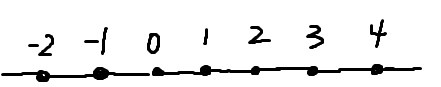
\includegraphics[width=\linewidth ,totalheight=0.95\textheight , keepaspectratio]{直线轴和整数系.png}
\caption{直线轴和整数系}
\end{figure}

如上图所示,向右移动的动作是加上某个数,数字一表示向右移动了一个单位距离,数字二表示向右移动了两个单位距离。2+1表示从数字点2向右移动了一个单位距离得到3,2+2表示从数字点2向右移动了两个单位距离得到了数字4。

显然这里讨论的绘图动作仅仅只是一种数学建模手段,数学只需要保证数字上计算的一切可能性得到保证即可,至于具体该数字最后映射到具体的某个动作,最后具体有什么含义那完全取决于数学工具使用者自身了。



\subsection{自然数减法}
那么如果是向左移动呢?

如果是向左移动那么就会得到减去某个数字的效果。比如5-1就是数字5向左移动一位得到数字4。

某些情况下减法最多只能减到0,比如3个苹果最多减到0表示没有剩下苹果了,再减下去就没有含义了。

但某些时候向左移动,一直减下去都是有含义的,比如说向右移动被解释为A向银行存钱,向左移动被解释为A向银行取钱,某些情况下是允许赊账的,这也是负数最早的应用实践。


\subsection{零和负数}
如果一种动作应用情景没有潜在的产生负数的可能性,实际上零这个数字也很大可能不会被发明出来,比如说分苹果,一堆3个苹果,分给你一个,还剩下2个苹果。这就是一个减法的应用,但这个应用情景最多只能减到0,没人对0个苹果和0个香蕉的区别在意,可能最多说没了,没有了,就完了。而用不到去发明那个纯粹的数字零。

因为有的动作应用情景有产生负数的可能性,需要记录这种状态,比如前面的和银行取钱赊账的例子,于是0和负数也一并被发明出来了。

负数是一个很抽象的概念,比有理数都抽象。有理数是1到10,现在假设10为1,那么之前的那个1就成了1/10,这个1/10记号和以前的数字1记号并没有区别,因为大家都知道底层逻辑仍然是1 2 3...这样的自然数序列。负数的抽象包含了两层,一层是实际负向动作的理解,另一层是在这个负向动作基础之上再去用自然数序列那一套逻辑来理解其中的数字。



\section{整数序列}
基于上一节的动作分析,人们发明了如下整数序列。

\begin{align*}
...\\
4 &\equiv 0 + 1 + 1 + 1 +1 \\
3 &\equiv 0 + 1 + 1 +1 \\
2 &\equiv 0 + 1 +1 \\
1 &\equiv 0 + 1 \\
0\\
-1 &\equiv 0 - 1 \\
-2 &\equiv 0 - 1 -1\\
-3 &\equiv 0 - 1 - 1 -1 \\
-4 &\equiv 0 - 1 - 1 - 1 -1\\
...
\end{align*}

关于这个整数序列的一些基本情况的描述,是一些恒等定义。

如果整数a大于0则称之为正整数,所有的正整数都比0大,记作 $a>0$ 。

如果整数a小于0则称之为负整数,所有的负整数都比0小,记作 $a<0$。

整数由零和自然数也就是正整数和负整数组成,其中负整数由负号和正整数值组合而成。

定义\emph{逆运算}:一个东西执行了一次运算和一次与之对应的逆运算,该东西状态不变。

对于任意整数来说,-1是+1的\emph{逆运算},执行一次-1动作再执行一次+1动作原整数不变。


\subsection{整数和它的相反数}
令a为一个整数,则-a叫做a的相反数。并有: 

\begin{equation}
(-(-a)) \equiv a
\end{equation}


\subsection{整数的方向符号}
上面的$+1$ 表示正向单元动作,比如在直线上向右移动一个单位距离; $-1$ 表示和正向单元动作相反的负向单元动作,比如在直线上向左移动一个单位距离。

这个方向符号结合在直线上的移动距离即某个正整数值组成成了整数。其中正整数比如$+5$一般会简写为$5$而省略其关联的正向符号。

为了下面讨论的方便,新增了一个 $+0$ 和 $-0$ 动作。并有如下恒等定义。

\begin{equation}
a +0 \equiv a
\end{equation}

\begin{equation}
a -0 \equiv a
\end{equation}

即任意整数无论加多少次零和减去多少次零都等于其自身。

\section{整数的一般定义}
整数可以分解为方向符号和正整数距离两个组成部分。

令a为任意整数,其内的正整数值为t,记为$t>0$ ,则整数a可以表示为:

\begin{align*}
if \quad a>0 \quad then \quad a=0+(+1+1+...)_t\\
if \quad a=0 \quad then \quad a=0+(+0+0+...)_t\\
if \quad a<0 \quad then \quad a=0+(-1-1-1....)_t
\end{align*}

现在令整数的符号$s$,$s$可能是+1,+0,-1这三个值,则整数a表示为:

\[
a = (sss...)_t
\]

\section{加上整数的一般定义}
加上某个整数$a$被定义为如下动作序列描述:

\begin{align*}
if \quad a>0 \quad then \quad +a=(+1+1+...)_t\\
if \quad a=0 \quad then \quad +a=(+0+0+...)_t\\
if \quad a<0 \quad then \quad +a=(-1-1-1....)_t
\end{align*}

即有

\[
+a = (sss...)_t
\]

方向符号s如果表示为-s,那么原为+1则变为-1,原为-1则变为+1,+0和-0都是一样的。

按照整数序列和加法定义继而有 $0+a = a$ ,零和任意整数相加等于该整数自身。


\section{减去整数的一般定义}
减去某个整数被定义为如下动作序列描述:

\begin{align*}
if \quad a>0 \quad then \quad -a=(-1-1...)_t\\
if \quad a=0 \quad then \quad -a=(-0-0...)_t\\
if \quad a<0 \quad then \quad -a=(+1+1+1....)_t
\end{align*}

\[
-a = (-s-s-s...)_t
\]

按照整数序列和减法的定义有:$0-a=-a$  ,0减去a等于该整数a的相反数。

上面第三行用到了【注意下面第一个符号是减去动作,和前面的 $(-(-1))$ 取两次相反数动作是有区别的】:
\begin{equation}
-(-1) = +1
\end{equation}

实际上这个运算规则并不是那么显而易见,不显而易见的意思在日常生活中会应用场景比较稀少,并没有那种经验直觉约束。一番尝试之后,这个只有根据减法是加法的逆运算这个原初定义推出来:

现在定义减法是加法的逆运算,以0来举例,令 $t=-(-1)$ ,那么有0减去-1再加上-1将保持不变:

\begin{align*}
0-(-1)+(-1)=0\\
t-1=0
\end{align*}

可以看到t必须等于1。所以有 $-(-1) = 1$。实际上也正是因为这里完成了证明,再加上前面的相反数的讨论,才有了减法符号和负数本身的取相反数符号可以不用区分而混为一谈的。

继而有任何整数a减去自身等于0。

\begin{equation}
+a -a \equiv 0
\end{equation}


\section{减法的含义}
任意整数a减去任意整数b在数轴上有特殊含义。其值的符号有:

\begin{align*}
if \quad a>b \quad then \quad a-b>0\\
if \quad a=b \quad then \quad a-b=0\\
if \quad a<b \quad then \quad a-b<0
\end{align*}

也就是说一个整数a大于一个整数b,那么a会在b的右边,a减去b得到的值会大于零。

减法等于 $a-b = s|a-b|$ ,s符号由上面描述的a和b之间的大小关系给出,$|a-b|$描述了a点和b点之间的距离,并有:

\begin{align*}
if \quad a>b \quad then \quad |a-b| = a-b\\
if \quad a<b \quad then \quad |a-b| = b-a
\end{align*}

上面的证明可以罗列各种情况来证明之,但多少过于繁琐了。

有了上面的讨论,如下等式即得到证明。

\begin{equation}
\label{eq:3.8}
a - b = -(b-a)
\end{equation}

\begin{align*}
b-a = s|a-b| \\
a-b = -s|a-b| = -(b-a)
\end{align*}


\section{整数下的加法交换律}
任意整数a和零相加符合交换律上面已经证得。

对于任意整数a和另外一个非零整数b相加的情况,如果a为零,参照上面,显然也是符合交换律的。

现在考虑a非零b非零的情况,a表示为 $a=(sss...)_t$ t>0,b如果和a符号相同,那么b为 $b=(sss...)p$ p>0 


\begin{align*}
a + b = 0 + a +b = 0 + (sss...)_t + (sss...)_p\\
=0+(sss...)_p + (sss...)_t\\
=b+a
\end{align*}

上面第二行是t个s和p个s,对应t个点和p个点,操作符号s都是一样的,所以换为p个点一堆和t个点一堆是一样的。

如果b和a的符号不同,那么b为 $b=(-s-s-s...)p$ 

现在假设p=1 ,符号操作有: $+s-s=0$ 

\begin{align*}
a + b = 0 + a +b = 0 + (sss...)_t + (-s)\\
=(-s) + (s) + (sss...)_{t} + (-s)\\
= (-s) + (sss...)_{t+1-1}\\
= (-s) + (sss...)_t\\
= b+a
\end{align*}

现在假设p=n的时候交换律 $a+(-s-s-s...)_n=(-s-s-s...)_n+a$ 成立的,下面是对n+1的情况讨论:

\begin{align*}
a + b = 0 + a +b = 0 + (sss...)_t + (-s-s-s...)_{n+1}\\
=(sss...)_{t} +(-s-s-s...)_{n} + (-s)\\
= (-s-s-s...)_{n} + (sss...)_{t} + (-s)\\
= (-s-s-s...)_{n} + (-s) + (s) + (sss...)_t + (-s)\\
= (-s-s-s...)_{n+1} + (sss...)_t\\
= b + a
\end{align*}

于是证得对于任意整数a和任意整数b符合加法交换律:

\begin{equation}
a+ b = b+ a
\end{equation}



\section{整数下的加法结合律}
\begin{equation}
a + b + c = a + (b + c)
\end{equation}

令$b=(sss...)_t$  如果b和c符号相同,那么 $c=(sss...)_p$

\begin{align}
a + (sss...)_t + (sss...)_p = a+ (sss...)_{t+p}\\
a + ((sss...)_t + (sss...)_p) = a+ (sss...)_{t+p}
\end{align}

对于整数a来说都是执行了相同的符号动作s,并执行了相同的次数,最终结果当然是相等的。

如果b和c符号不同,那么 $c=(-s-s-s...)_p$

\begin{align}
a + (sss...)_t + (-s-s-s...)_p = a+ (sss...)_{t-p}\\
a + ((sss...)_t + (-s-s-s...)_p) = a+ (sss...)_{t-p}
\end{align}

对于整数a来说都是执行了t次s动作再执行了p次-s动作,最后结果当然是相同的。

\section{整数下的乘法}
\subsection{零和乘法}
不管是零个某个东西还是多少个零都是零,这是很显而易见,但还是写出来:

\begin{equation}
a * 0 \equiv 0 * a \equiv 0
\end{equation}

乘法的一些运算规律显然都是成立的。

\subsection{负数和乘法}
负数实际上是负向符号和自然数的组合,按照前面乘法定义分析,是只能接受自然数乘以某个东西的情况。所以说 $-5*1$ 负5个1,这样的说法本来是没有含义的,这就是数学家们自由发挥定义的领域了。

出于乘法交换律的考虑 $-5*1=1*-5$ ,一个-5倒是有自然语境约束,最好还是等于-5。所以对于负数乘以正整数的情况,是负号保留,其余正数值相乘。

而对于 $-5*-1$ 这样的情况,\cite{什么是数学}介绍到,这是出于乘法分配律的考虑。比如

对于任意的负数 $-n$ 和任意的正整数a

\begin{align*}
-n * (a-a) = -n * a - (-n)*(-a) =0\\
=-n*a - ? =0
\end{align*}

也就是负数和负数相乘,得数为正,具体值为各个负数的正数值相乘。

所以本小节讨论的负数的乘法行为,都是数学家们定义出来的,为了就是满足人们在运算中熟悉的那一套运算规律。

\subsection{整数的乘法的一般定义}
a为任意整数,表示为 $s_a(t_a)$ ,s是其符号,t是其正数值。b为任意整数,表示为 $s_b(t_b)$ 

\begin{align}
a * b = (s_a*s_b)(t_a*t_b)
\end{align}

其中符号s的运算规则如下:

\begin{itemize}
\item $+1*+1 = +1$
\item $+1*-1 =-1$
\item $-1*+1 = -1$
\item $-1*-1 = +1$
\end{itemize}

如上符号s的运算规则四个,一观察就能得出结论,符号s的运算符合交换律,即计算结果和顺序无关。


\subsection{整数下的乘法交换律}
a为任意整数,表示为 $s_a(t_a)$ ,s是其符号,t是其正数值。b为任意整数,表示为 $s_b(t_b)$ 

\begin{align*}
a*b =  (s_a*s_b)(t_a*t_b)\\
(s_b*s_a)(t_b*t_a)\\
b*a =  (s_b*s_a)(t_b*t_a)\\
\end{align*}

这样就证得了:

\begin{equation}
a * b = b * a
\end{equation}


\subsection{整数下的乘法结合律}
对于任意整数a,b,c 有:

\begin{equation}
a * (b * c) = (a * b) * c
\end{equation}

\begin{align*}
a * (b * c) = s_a(t_a) * ((s_b*s_c)(t_b*t_c))\\
= (s_a*s_b*s_c)(t_a*t_b*t_c)\\
(a * b) * c = s_c(t_c) * ((s_a*s_b)(t_a*t_b))\\
= (s_a*s_b*s_c)(t_a*t_b*t_c)
\end{align*}


\subsection{整数下的乘法分配律}
a,b,c为任意整数,整数下的加法结合律已经证得,a如果是自然数的情况,乘法分配律已经证得。

现在主要需要证明a是负数的情况,令$a=-n$ ,n为任意自然数。

\begin{align*}
a*(b+c) = -n*(b+c) = -1*n*(b+c) = -1*(n * (b+c))\\
-1 * (n*b+n*c)\\
-n*b + -n*c\\
a*b + a*c
\end{align*}

上面第二行用到了整数下的乘法结合律。

第三行看起来不太明显,需要证明:

a,b是任意整数:
\begin{align*}
if \quad a+b > 0 \quad then \quad -1 * (a+b) = (-1*1)|a+b|\\
= -1(a+b) = -a - b \\
if \quad a+b <0  \quad then \quad -1 * (a+b) = (-1*-1)|a+b|\\ 
= 1(-a-b) = -a-b
\end{align*}
上面第一行第三行用到了乘法的一般定义。

第二行第四行用到了 (\ref{eq:3.8})

于是证得:
\begin{equation}
\label{eq:4.10}
-1 * (a+b) = -a -b
\end{equation}

因为现在还在证明分配律,所以不能直接展开,上面实际上已经证明了:

t是任意整数:
\begin{align*}
if \quad t > 0 \quad then \quad -1 * (t) = (-1*1)|t|\\
= -1(t) = -t \\
if \quad t <0  \quad then \quad -1 * (t) = (-1*-1)|t|\\ 
= 1(-t) = -t
\end{align*}

即对于任意整数a有:

\begin{equation}
\label{eq:4.11}
-1 * a = -a
\end{equation}

即$-1$ 乘以任意整数 $a$就可以直接简写为 $-a$ 了。

\subsection{一个小应用题}
a,b,c,d是任意整数,证明:

\begin{equation}
(a-b) * (c-d) = ac - ad - bc +db 
\end{equation}

\begin{align*}
(a-b) * (c-d) = (a-b) * c + (a-b) *(-d)\\
= c*(a-b) + (-d) * (a-b) \\
= c*a  - c*b -d*a + d*b\\
= ac -ad -bc +db
\end{align*}

上面主要是乘法分配律和交换律的应用,此外还有 (\ref{eq:4.11}) 。

\section{整数下的除法}
整数下除法,主要是负数的引入,这种情况甚至到了现在数学上也没有规范,一些编程语言也有各自不同的解释。你也不能说它们错了,数学上对于整数下的除法,唯一的要求就是它必须符合:

\[
a = n*b + r
\]

即由除法得到的商乘以除数再加上余数一定要等于原来的被除数。

python中商是通过 \verb+a//b+ 来获得的,更确切来说是 \verb+floor(a/b)+ ,而取模也就是求余数是 \verb+a % b+ ,更确切来说是\verb+a - floor(a/b)+ 。JavaScript在负数整除商行为就和python略有差异。



\chapter{有理数}
\section{单位分数的引入}
对 \cite{古今数学思想} 描绘的人类早期数学样貌进行分析,就会发现分数出现的非常早,极端的情况下自然数序列都还没发展好,一些大的数字都还不能表达,但已经有 $\frac{1}{2}$ 、$\frac{1}{3}$ 这样的分数了。

\cite{高观点下的初等数学第一卷} 提到了分数的两种现代解释:一种是分数仅仅只是一个记号,整数组成的一个数偶,具体其运算法则是一些约定;另一种解释是分数是整数域内先乘以a再除以b的一个运算序列。第二种解释更像是一种结果,也就是为什么分数可以解释为这样的运算序列是一个待证明的结论,而不应该成为分数的原初定义。第一种解释更合乎历史真相,不过有很多细节需要讨论,这就是接下来要做的。

再开始之前,先介绍一下古埃及人是如何计算19除以8的,他们的算法,头脑中进行的动作,很值得细细品味:

\begin{align*}
&2   &  &1   &  &1/2  &  &1/3  &  &1/4  & &...   &1/8\\
&16 &   &8    &   &4  &   &?       &  &2     &  &...  &1
\end{align*}

因为$3*8=24>19$ 所以19除以8得商为2,余数为3,在自然数的除法这点上古埃及人和现在没有区别,古埃及人似乎是为了解决不能整除的问题,引入了分数。并且对于分数已经有了这样的认识。

\emph{单位分数} $\frac{1}{n}$ 的含义就是将一个东西分成n份\footnote{他们的符号标记语言还不如现代发达规范,这里只讨论他们头脑中所理解的东西。}。

并有如下恒等定义:
\begin{align}
n * \frac{1}{n} \equiv 1
\end{align}

如下单位分数序列越来越小:

\[
\left\{\frac{1}{2} \quad \frac{1}{3}  \quad \frac{1}{4} \quad  ...  \quad \frac{1}{n} \right\}
\]

所以现在的问题就是要表达数字3为8的某个倍数,然后发现 $\frac{1}{4} * 8 = 2<3$ ,所以19除以8可以更精确地表达为 $2 + 1/4$ ,然后还有余数1。最终古埃及人发现19除以8得到 $2 + 1/4 + 1/8$ 没有余数。

古埃及人利用上面的单位分数概念进而发展出一套复杂的做法,来对分数进行四则运算,这套做法和现代习惯的分数运算规则有很大区别,后面将会讨论到其具体细节。之所以会这样是因为现代习惯的那些分数运算规则里面有些是数学家的发明创造,并不是那么显而易见,不是一定要这样的。古埃及人在这方面没做对,造成了他们的分数运算非常的繁复,这一定程度上阻碍了他们的数学的进一步发展。
 

\section{分数的动作分析其一}
本小节的内容初看会觉得很抽象,我有好几次想将其删去,因为本小节的内容,是存在一定的猜想成分的。但最终还是决定不那么做,是因为我觉得,现在需要去强调这样一个观念,那就是人们习以为常的分数,其底层逻辑也是以智能体的动作为基础的。虽然我已经取消了将乘法和除法也建立在分数动作的基础上的极端猜想\footnote{似乎有点逆反,对将分数简单看作乘除法的批判。},但分数的底层动作逻辑和乘除法的识别动作逻辑又是有所不同的,这也是需要强调的一个点。

本小节讨论的数如果是初次阅读可以认为是自然数\footnote{如果是第二次阅读那么应将这里数理解为正有理数,即一个更广义上的自然数。},负数只是额外多了一个记号标记了负向动作,并不影响该动作其内数值的缩放动作的讨论。

数对于智能体来说\footnote{只有人类才进化出了把数看作某种符号的能力,但对于其他大部分智能体来说,数是具现的。},本身就是和其内部表达某个东西或者某个动作绑定在一起的。智能体为了模拟外部世界,来更好地理解外部世界,和外部世界交互,当然是需要实现类似的数上的变化。

对于模拟外部世界这样的数变化的需求,物的同一性要求智能体内部具有某种数的缩放动作SM,对于某个东西 $p(x)$,发生缩放动作之后,令其得到另外的某个东西 $q(x)$ 即:

\[
p(x) \to q(x)   
\]

如果$p>q$ ,那么这个缩放动作的效果就是数字的缩小;如果 $p<q$ ,那么这个缩放动作的效果就是数字的放大。

缩小动作的q最小只能到1,于是缩小动作S(p,1,x)描述的是某个东西的最小部分;放大动作的p最小只能到1,这也是所谓的除法不能除以0,或者0不能作为分母的缘由。

上面的描述认为最小的那个东西为x,然后当前研究的东西为 $p(x)$ ,缩小动作之后东西为 $q(x)$ ,这样描述是为了方便理解。但人们一般会将当前研究的东西认为是一个东西,于是人们发明了这种写法$\frac{1}{p}(x)$ 来表示某个东西x的最小组成部分,这样$q(x)$就变成了 $q(\frac{1}{p}(x))$ ,而当前研究的某个东西就成了人们习惯的x,即上面的缩放动作改写为:


\[
x \to q(\frac{1}{p}(x))  
\]

上面的那个东西 $q(\frac{1}{p}(x))$,大体就是分数了,按照上面对于分数的描述有:

\begin{equation}
p(\frac{1}{p}) \equiv 1
\end{equation}

这也是分数之所以被认为是一个数的原因,那只是因为人们习惯了12个鸡蛋形容为一打,所以一个鸡蛋才会被记作 $\frac{1}{12}$ 打。但如果从最小的鸡蛋视角来看,看到的仍然是1 2 3...这样的自然数序列,在那里, $\frac{1}{12}$ 打就是对应的那个数字1个鸡蛋。



\section{分数}
缩放动作

\begin{equation}
SM(p,q,x) = q* \frac{1}{p} *x
\end{equation}

现在令x是一个纯粹的数,那么缩放函数S(p,q,n)的输出就是将分数 $q* \frac{1}{p}$ 乘以该自然数n。

人们会将 $q* \frac{1}{p}$ 缩写为 $\frac{q}{p}$ ,即:

\begin{equation}
\frac{q}{p} \equiv q* \frac{1}{p}
\end{equation}

按照上面的讨论有\emph{分数}:$\frac{q}{p}$ ,是这样一个数,其乘以某个数的效果就是将该数缩放为原来的 $\frac{q}{p}$ 。


令 $p=\aleph_0$ ,则该东西的可能缩小比为:

\[
\left\{1 \quad \frac{\aleph_0-1}{\aleph_0} \quad \frac{\aleph_0-2}{\aleph_0} \quad  ...  \quad \frac{1}{\aleph_0} \right\}
\]

举一个具体的例子,令$\aleph_0 = 5$ ,则有:

\[
\left\{1 \quad \frac{4}{5} \quad \frac{3}{5} \quad  \frac{2}{5}  \quad \frac{1}{5} \right\}
\]

现在定义 $\frac{1}{\aleph_0}$ 为这个东西的\emph{极限小}。

由极限小组成的可能性集合如下:

\[
\left\{1 \quad \frac{1}{2} \quad \frac{1}{3} \quad  ...  \quad \frac{1}{\aleph_0} \right\}
\]


上面的序列一直类推下去将会得到 \emph{无限小}的概念。但无限小只是一个推理抽象出来的产物,不一定有实际含义。

\subsection{分数的乘法}
如下说明清楚单位分数的乘法行为即说明清楚分数的乘法行为了。

\subsubsection{单位分数的乘法}
对于分数的乘法有(a,b为任意整数,不能为0):

\begin{equation}
\label{eq:17}
\frac{1}{a*b} = \frac{1}{a} * \frac{1}{b}
\end{equation}

\begin{align*}
\frac{1}{a*b} * (a*b) &=1\\
&= (a*\frac{1}{a}) * (b * \frac{1}{b})\\
&=(\frac{1}{a} * \frac{1}{b}) * (a*b)
\end{align*}

上面证明用到了分数的定义恒等形式 $p\frac{1}{p} \equiv 1$ 和乘法的结合律。但是注意这个 $\frac{1}{a}$ 并不是整数,现在我们手头上只有整数下的乘法是符合结合律的。似乎是人们在心里就默认 $\frac{1}{a}$ 这个东西是一个整数,这倒也是很合理的一个假设。

但如果连分数的乘法行为都没有,就声明证明了分数的乘法符合结合律,这是很奇怪的。所以数学家们认为更严格的说法是分数的乘法,上述行为是被定义出来的,这种定义如上是为了让其符合乘法的结合律。



\subsection{分数的加法}
\subsubsection{分数消去公因数}
公因数也叫公约数,具体到这里就是指能够同时整除分子和分母的数。

\begin{align*}
\frac{a*c}{b*c} &\equiv (a * c) * \frac{1}{b*c}\\
&=a * c * \frac{1}{b} * \frac{1}{c}\\
&=a*c*\frac{1}{c}*\frac{1}{b}\\
&\equiv a*\frac{1}{b}\\
&\equiv \frac{a}{b}
\end{align*}

第二行用到了 (\ref{eq:17})

第三行乘法交换律【待证明,或者说为了满足乘法交换律而定义的分数的这个消去公因数行为。】

\subsubsection{分数分子的拆分}
\begin{align*}
\frac{a+b}{c} &\equiv (a+b) * \frac{1}{c}\\
&=a* \frac{1}{c} + b* \frac{1}{c}\\
&\equiv \frac{a}{c} + \frac{b}{c}
\end{align*}

第二行用到了分配律。【待证明,或者说为了满足乘法分配律而定义的这个行为】


基于上面的讨论,于是有分数的加法是:
\begin{align*}
\frac{1}{a} + \frac{1}{b} = \frac{b}{ab} + \frac{a}{ab}\\
= \frac{a+b}{ab}
\end{align*}

\section{有理数下的运算律}
下面会证明有理数的一些基本运算律,可以简单看下。在对分数的加法和乘法进行讨论的时候实际上已经预先假设分数是符合乘法分配律、乘法交换律和结合律的。

\subsection{有理数下的加法交换律}
令有理数 $a = \frac{q_a}{p_a}$ 其中p,q为任意整数,此外还限定 $p \neq 0$ 。

令有理数 $b = \frac{q_b}{p_b}$ 其中p,q为任意整数,此外还限定 $p \neq 0$ 。


\begin{align*}
\frac{q_a}{p_a} + \frac{q_b}{p_b} = \frac{q_a *p_b}{p_a * p_b} + \frac{q_b * p_a}{p_b * p_a}\\
= \frac{q_a * p_b + q_b * p_a}{p_a * p_b} \\
= \frac{q_b * p_a + q_a * p_b}{p_a * p_b} \\
= \frac{q_b*p_a}{p_a*p_b} + \frac{q_a * p_b}{p_a * p_b}\\
= \frac{q_b}{p_b} + \frac{q_a}{p_a}
\end{align*}


\subsection{有理数下的加法结合律}
令有理数 $a = \frac{q_a}{p_a}$ 其中p,q为任意整数,此外还限定 $p \neq 0$ 。

令有理数 $b = \frac{q_b}{p_b}$ 其中p,q为任意整数,此外还限定 $p \neq 0$ 。

令有理数 $c = \frac{q_c}{p_c}$ 其中p,q为任意整数,此外还限定 $p \neq 0$ 。


\begin{align*}
a + b + c = \frac{q_b * p_a + q_a * p_b}{p_a * p_b} + \frac{q_c}{p_c}\\
=\frac{q_b*p_a*p_c + q_a*p_b*p_c + p_a*p_b*q_c}{p_a*p_b*p_c}\\
a + (b + c) =  \frac{q_a}{p_a} + \frac{q_c * p_b + q_b * p_c}{p_b * p_c}\\
=\frac{q_a*p_b*p_c + p_a*q_c*p_b + p_a*q_b*p_c}{p_a*p_b*p_c}
\end{align*}

简单对比下就会发现是一样的,所以有:

\begin{equation}
a + b + c  = a+(b+c)
\end{equation}



\subsection{有理数下的乘法交换律}
令有理数 $a = \frac{q_a}{p_a}$ 其中p,q为任意整数,此外还限定 $p \neq 0$ 。

令有理数 $b = \frac{q_b}{p_b}$ 其中p,q为任意整数,此外还限定 $p \neq 0$ 。

\begin{align*}
a * b = \frac{q_a}{p_a} * \frac{q_b}{p_b}\\
= \frac{q_a * q_b}{p_a*p_b} \\
b * a =  \frac{q_b}{p_b} * \frac{q_a}{p_a} \\
= \frac{q_a * q_b}{p_a*p_b} 
\end{align*}

上面因为都是整数,自由使用交换律。

\begin{equation}
a * b = b * a
\end{equation}


\subsection{有理数下的乘法结合律}
令有理数 $a = \frac{q_a}{p_a}$ 其中p,q为任意整数,此外还限定 $p \neq 0$ 。

令有理数 $b = \frac{q_b}{p_b}$ 其中p,q为任意整数,此外还限定 $p \neq 0$ 。

令有理数 $c = \frac{q_c}{p_c}$ 其中p,q为任意整数,此外还限定 $p \neq 0$ 。

\begin{align*}
a * b * c = \frac{q_a}{p_a} * \frac{q_b}{p_b} * \frac{q_c}{p_c}\\
= \frac{q_a * q_b * q_c}{p_a*p_b*p_c} \\
= a * (b *c)
\end{align*}



\subsection{有理数下的乘法分配律}
令有理数 $a = \frac{q_a}{p_a}$ 其中p,q为任意整数,此外还限定 $p \neq 0$ 。

令有理数 $b = \frac{q_b}{p_b}$ 其中p,q为任意整数,此外还限定 $p \neq 0$ 。

令有理数 $c = \frac{q_c}{p_c}$ 其中p,q为任意整数,此外还限定 $p \neq 0$ 。


\begin{align*}
a * (b + c) = \frac{q_a}{p_a} * ( \frac{q_c * p_b + q_b * p_c}{p_b * p_c})\\
= \frac{q_a*q_c*p_b + q_a*q_b*p_c}{p_a*p_b*p_c}\\
= \frac{q_a*q_c}{p_a*p_c} + \frac{q_a*q_b}{p_a*p_b}\\
=\frac{q_a}{p_a} * \frac{q_c}{p_c} + \frac{q_a}{p_a} * \frac{q_b}{p_b}\\
= a*b + a*c
\end{align*}


\section{有理数和数轴}
现在在整数和数轴的讨论基础上,又多了很多有理数点。

\begin{figure}[H]
\centering
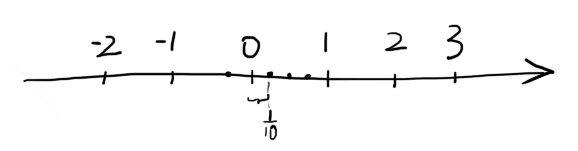
\includegraphics[width=\linewidth ,totalheight=0.95\textheight , keepaspectratio]{数轴和有理数系.png}
\caption{数轴和有理数}
\end{figure}

在数轴上,随便取一个数据点,对那个数据点加上一个正数值,意思就是这个点向右移动了一定的距离。如果减去一个正数值,那么就是由这个点向左移动了一定的距离。

现在有了分数和乘法,从而实现了数的缩放动作,可以实现这个数据点对于任何其他一个有理数点的跳跃动作。

类似整数的讨论,有理数在数轴上同样有越靠右边,其数越大的规律。并有 $a-b>0$ ,那么有理数a大于有理数b,有理数a在b的右边。

任意选中的两个有理数构成一个区间 $[A, B]$ ,这个区间之内仍然可以找到另外一个有理数,这称之为有理数在数轴上是稠密的。


\subsection{等式运算规则其一}
a,b是任意有理数,c为任意有理数,则有:

\begin{equation}
a+c = b+c \Leftrightarrow a=b
\end{equation}

a,b是数轴上相同的某个点,那么它们经由有理数c描述的相同的移动动作,最终仍然会落在相同的某个有理数点上。


\subsection{等式运算规则其二}
a,b是任意有理数,t是任意的有理数,$t \neq 0$ :

\begin{equation}
a*t=b*t \Leftrightarrow a=b
\end{equation}

a,b是数轴上相同的某个点,那么它们经由有理数t描述的相同的缩放动作,最终仍然会落在相同的某个有理数点上。

\section{有理数域}
所有有理数构成的 \emph{有理数集}  $ \mathbb{Q} $,在有理数集下,进行有理运算,也就是通常所说的四则运算,加减乘除,其值仍然处在有理数集中。并有上面描述的有理数下的加法交换律、加法结合律、乘法交换律、乘法结合律、乘法分配律成立。并且方程 $a + x = b$ 和 $a*x=b$ 总有解 $x = b-a$ 和 $x = b/a \quad a\neq 0$ ,这样一个封闭的数的集合,称之为域,有理数就是一个域,即有理数域。

 
\subsection{有理数域下的代数动作}
现在有恒等式, $t=f(a, b)$ ,其中t数的所有可能集合是有理数集,a数和b数的所有可能集合也是有理数集, $f(a,b)$ 这个表达式里面只有加减乘除四种运算,那么按照有理数域的定义,$f(a,b)$ 的可能的值的集合也是有理数集。

所以对于其他任何的表达式,只需要证明 $t=f(a,b)$ 这个等式为真,就可以执行代数动作了。注意这里说的是其他任何表达式,也就是有理数t在其他一个你没见过的表达式里面,只要满足上面讨论的条件,就可以执行 $t=f(a,b)$ 代数动作。



\chapter{有理数补充}
\section{十进制}
实践中,对于很大的数和很小的数,都需要一种方便的表示方法,这里只讨论十进制的情况。

以 $683.979$ 举例,其具体含义为:

\[
683.979 = 6*100 + 8 * 10 + 3 + 9*\frac{1}{10} + 7 * \frac{1}{100} + 9 * \frac{1}{1000}
\]

这一连串数字可以理解为人们用100米的尺子测量,取整得到数字6,剩下的部分不足100米一个单位了,然后用10米的尺子继续测量,得到数字8等等等等,最后用了 $\frac{1}{1000}$ 米的尺子测量,可能还剩下来一点,但人们已经不关心了。

除法可以看作乘法的逆运算,也可以看作某个数字乘以某个单位分数,也可以看作对某个数连续执行被除数的减去动作等等,但不要对除法太过于热心,总是热衷于要将 $1/3$ 不停地除下去,$1/3$ 就是确定的一个数字了,和数字1一样没有区别,别用除法或者小数来看,然后觉得它好像是一个另类。

小数的目的就是一种方便的表示方法,更贴近真实的测量动作,除法在其中的目的就是通过上面描述的动作过程来获取小数这样一种便捷的表示。当用 $0.333$ 来表示 $1/3$ 的时候,只是人决定给这个东西换一个名字,不影响不改变其他任何东西。

十进制小数进行运算比分数方便,尤其是在工程项目中有大量运算的场景下。一般来说这样的小数运算是一种近似运算,很少有这样的情况是 $1/8$,也就是 $0.125$ ,更常见的情况是:也许理论值是 $1/3$ ,但用 $0.333$ 来近似运算;也许测量的结果在 3.14米到3.15米之间,就在刻度线4厘米到5厘米之间的某个位置等等。有关近似运算的讨论下面会专门开一章分析。


\section{浅谈无理数}
无理数这个概念是理论数学研究的领域,对于大部分人们来说,本小节讨论的内容,简单了解下即可。

\cite{高观点下的初等数学第一卷}首先说明了在应用上,任何测量获得的值必然是存在某个极限的,超过这个极限下面的一些小数位数里面的数字是没有意义的;此外从实践,比如说计算机的角度出发,实践中数字的表示也是存在一个极限的。

\begin{bookref}[frametitle={\cite{高观点下的初等数学第一卷}}]
可以将数学分成两部分,称之为近似数学及精确数学。以解方程 $f(x) = 0$来说明这个区别,近似数学,并不关心$f(x)$ 是否正好等于零,只关心 $|f(x)|$ 恒在可达到的精确性的阈值 $\eta$ 以下。符号$f(x)=0$ 仅为不等式 $|f(x)| < \eta$ 的简写。只有在精确数学,才不折不扣地要求$f(x)=0$ 。


无理数的概念当然只是精确数学范围内的概念。
\end{bookref}

假设当前的科学发展水平下,对于目标问题获得的数值的有效数字位数为k,那么任何实数x都需要表达成如下近似值。

\[
\frac{E(10^k x)}{10^k}
\]

上面的E函数是一个取整函数。所以最终应用实践中,处理的都是一些有理数。

在实践中无理数也会用十进制小数来表示,从而进行的也是一种近似运算,有关近似运算的讨论下面会专门开一章分析。

\section{计算机中数的表示}
现在俯拾皆是的计算设备,关于数的基本运算,很多经典的形式化的证明结论已经变得不是那么重要了\footnote{当然读者如果有闲情逸致,就个别问题活跃下大脑,也是可以的。},对于大多数人来说,现在更重要的是弄明白计算机中的数是如何表示和计算的,然后利用这个工具解决对应的问题即可。

不同的计算机,不同的编程语言情况略有差异,但大体计算机将整数和浮点数分开来表示。

\subsection{整数}
python中的整数是 \verb+int+ 类型,有正负号,即上面讨论的整数,具有无限的精度,但存在一个最大的整数限制,超过了会抛出异常。

传统数学上很多只适合正整数领域的内容,因为计算机整数默认包含负数,很多概念进行了推广,并越来越成为一种惯例。

比如说-2是不是偶数,传统意义上的偶数是只讨论正整数内的,现在人们越来越接受-2也是偶数这个惯例约定了。



\subsection{浮点数}
对于计算机内的浮点数,一些不太严谨的著作会将它们叫做实数,但这是不正确的,也不能称之为是某种有理数,更好的称呼是类似纸面上存储的十进制小数的形式存储在了计算机里面,其内进行的也是一种近似计算。有关近似运算的讨论下面会专门开一章分析。

python中的浮点数基于C语言实现,可参考 \href{https://www.open-std.org/jtc1/sc22/wg14/www/docs/n1256.pdf}{C99} 里面的5.2.4的float标准 。

下面以十进制小数3.1415,并以十进制作为基底来举例,具体只是计算机用了二进制,简单类比一下即可。

\begin{align*}
s \cdot 0.31415 \cdot 10^m\\
+1 \cdot 0.31415 \cdot 10^1
\end{align*}

上面s是符号,具体到例子是+1,上面m是十进制的指数,具体到例子是1。

计算机进行小数的近似运算,每进行一步近似运算都会执行一次截断操作,即使是纸面运算,也不会小数后面位数全部算完,而是有效数字后面的位数也会直接丢弃,计算机在这里有类似的处理,可以认为计算机里面的有效数字位数就是它的尾数长度(就是上面31415这一串整数的符号位数),类似的误差估计应该也是可以类似处理,但这块内容在后面近似运算中再做详细讨论。


\section{分数的动作分析其二}
分数实现了对数的缩放,如果仅仅只是把一个点映射为两个点,怎么看也都不是什么了不起的事,但如果将这种数的映射变化再结合智能体自身的行动能力,那就彻底打开了智能体行为模式的多样性魔盒了。比如说对a物体识别为1,执行分数映射,产生2并封装动作走路,得到行为走两步。对于行为层面的技术细节,我不想在这里讨论太多,下面继续侧重数学方面的内容分析。请看下面这个数字序列:

\begin{align*}
1 \quad 2  \quad 3 \quad ... \\
2 \quad 4  \quad 6 \quad ...
\end{align*}


智能体(参考前面的分数消去公因数的讨论)最终将会发现,这些数具有相同的缩放比,也就是它不需要再创建那么多的行为单元了,只需要一个行为单元,该行为单位保持那个缩放比,然后对目标对象逐个执行分数缩放即可。

相同的缩放比是一个很重要的观念感受,将会在各个智能体的行为模式中反复出现。


\subsection{对蜘蛛结网的沉思}
现在假设我是一个蜘蛛,我该如何结网。结网的最终效果就是这个网由粘液点和丝线组成,粘液点的作用一方面是粘贴丝线,另一方面就是预备粘昆虫。结网的子动作构成如下:

\begin{enumerate}
\item 粘液点A拉丝到粘液点B,这将构成一根直线段【直线段的定义就是两个点用线连接起来,同时连接线是均匀的紧凑的。】。
\item 再从粘液点A移动到粘液点B,保持某个固定的缩放比,比如行走几步,滴下一滴粘液,如此重复行动到粘液点B。
\item 再从粘液点A拉丝到新的粘液点C,从而形成一根新的直线段,蜘蛛会先执行一个转向动作,这个转向动作确立了新的直线段和之前的那根有个夹角。并重复上面步骤2。
\item 重复上面步骤3,转向动作由相同的缩放比控制。
\item 将各个直线段从内到外各个粘液点用丝线连接起来,为了保证这个连接动作是从内到外的,蜘蛛在每连接动作一次之后都会执行一次微小的转向动作,这个转向动作是由固定的缩放比控制的。
\end{enumerate}

笔者没有对蜘蛛结网进行过研究,就算真实的某种蜘蛛是不同的也不影响上面的讨论,上面的讨论主要目的是展示相同的缩放比在智能体行为模式中的应用。



\subsection{缩放比的其他表述}
相同的缩放比因为智能体的各个行为的不同,有眼睛看的,有水平走路加向上登使劲动作等等,而采用不同的词语来表达某两个数值之间的相同的缩放比例关系。

比如眼睛看到一条直线,是因为这条直线在眼睛感知动作上,形成了某个固定的数值缩放比。

比如山坡的陡峭程度,是因为水平走路使劲和向上登使劲这两个动作上的数值缩放比,某个均匀的斜坡人们会感知到这两个数值具有相同的固定缩放比。

智能体在行为上只要某两个动作同时发生,并且具有数值上相同的缩放比,智能体就会敏锐地感知到。【内部技术实现细节上可能会发生某种置换合并动作,来更好地记忆和将来更节能地运算。】


\subsection{从直线到曲线}
很多人介绍微积分会用各种高大上的目的,但牛顿发明微分学目的只有,那就是理解曲线,而且手段也就是用直线来理解曲线。也就是将曲线看作一系列微小的直线拼接起来的,这样就能够计算得到曲线某个位置上的x和y这两个东西的缩放比(即斜率)。

物理上的计算出来的斜率一般有特殊的含义和需求,但数学上对一般函数的求导,也就是得到该函数在各个不同的地方的斜率组成的新的函数,会是更加泛泛而谈的。这个时候如何理解计算得到的导数,一般会建议从斜率或者山坡的陡峭度来理解,但笔者更加建议以一种,脱离几何空间感知的观念,将其视作两种同时发生的动作,不建议额外假设认为这两种动作存在因果关系,仅仅是这两种动作,碰巧同时发生了,然后这个地方的导数,是这两个动作在此处的数值缩放比。

也就是缩放比的理解必须将这两个数字映射为某种具体的两个动作,所以导数的理解也是如此。

数字本身没有含义,导数也没有含义,那种纯数学上的导数含义的解释看起来似乎说了点什么,学生也听了,但其实什么都没有说。必须将数字和具体的动作【这里不再说某个东西,因为涉及到变化这里必须是动作】结合起来,所以导数的理解根据具体的情况是仁者见仁智者见智的。

从爬坡运动的角度,假设人在爬某个曲线坡,暂时先抛开人的大小之类的因素不谈,就一般的爬坡而言,假设这个时候我们说此处斜率为5,意思就是告诉大腿,向上登的力设置为5N,告诉脚,水平行走的力设置为1N。



\subsection{转的角度}
智能体在两个直线段绘制动作之间,如果插入一个转向动作,来更改自己的某些状态,那么将会产生一根新的直线段。

这个转向动作附带的数,即这个转向动作的强度称为所转的角度。

在平面几何中,这个转的角度即这两根直线段所形成的夹角。

如果智能体所转角度为n之后发现绘制的新的那根直线段等于原来的那根,那么称这个角度为周角度。

在平面几何中,所转一周的角度等于 $360^{\circ}$ 。





\chapter{近似计算}
\section{小数运算是近似运算}
有理数就是一个确定无疑的数,同样无理数也是一个确定无疑的数,而智能体在观测外部世界中进行的各种测量活动,测量对象的目标属性值也是一个确定无疑的数。这种确定无疑是数学模型层面上的,到了实际情况,会有各种原因\footnote{这些原因前面提到过许多了,这里不再赘述了。},来将上面讨论的数转变为一种小数形式,这种小数形式是对上面准确数值的一种估计,这些小数被称之为近似数值\footnote{准确数值化为小数数值,有些情况比如说$ 1/8 $ 是可以除尽的,这只是很少见的个别情况,对于这些情况,更好地描述是近似数值恰好后面几位是几个零。},对这些小数进行的运算,或纸面上,或计算机上,统称为近似计算。

这样的近似计算通常是存在一系列的步骤的,这一系列步骤统称为近似计算过程。近似计算过程最开始的数据称为近似计算过程输入数据,近似计算过程最终的结果称之为近似计算过程输出数据。

\begin{figure}[H]
\centering
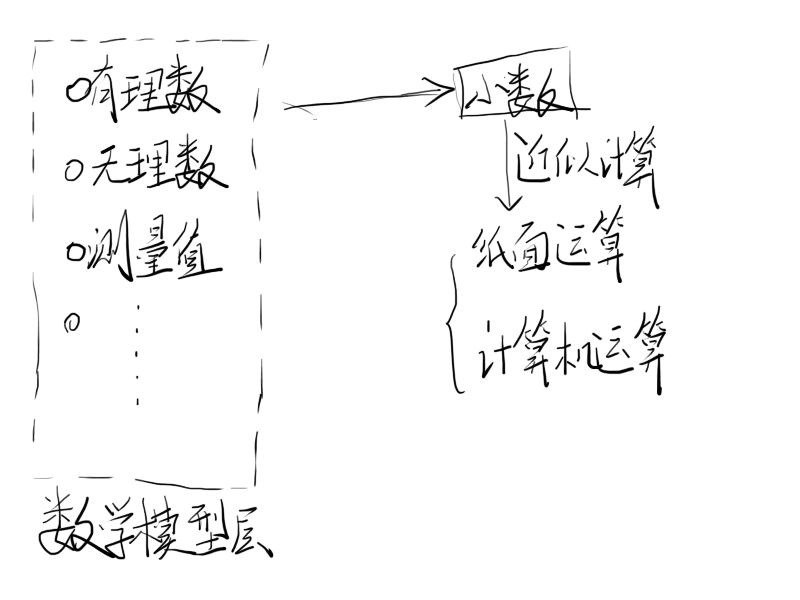
\includegraphics[width=\linewidth ,totalheight=0.95\textheight , keepaspectratio]{小数运算是近似运算.png}
\caption{小数运算是近似运算}
\end{figure}

近似计算它首先就是人们在计算或者计算机在计算时的真实面貌。对于这个真实面貌的正视,能够让人们更好地使用数学这个工具。

其一最直接的应用,近似计算可以加速计算,对于数据在复杂运算过程中,假设你拥有惊人的近似计算准确度直觉,那么在某些地方将节省大量的计算开销和存储开销,而输出结果不受影响。

第二个应用就是个人目前的一点遐想,包括某些神经网络局部结构,都可以看作某种近似计算过程 $f(x)$,如果近似计算过程随着给定输入区间的缩小,输出的区间也相应缩小,那么这个近似计算过程是稳定的,良态的。如果不是则称这个近似计算过程是混沌的。

显然混沌计算过程是不可以用反向误差传播也就是结果约束来规范限定出来的,这种计算过程,只可能通过某种进化算法,也就是智能体已经判断出这部分计算是混沌的,并将这部分计算隔离开来,使之成为单独的某部分,并试着从中获取有用的信息,在资源富裕的情况下,会容忍这些混沌计算过程存在,如果资源比较紧张,则会将其整个移除掉。



\section{获得近似计算区间}
在实践中,关于模型理论值 $A$ ,在穷极一些可能的信息之后,得到它的一个可能存在其中的估计区间: $[A_0, A_1]$ ,这个估计区间称之为近似计算区间。

对于一个良态的近似计算过程来说,严格的做法是应该取一个近似计算区间,这个近似计算区间总是确保准确数值在其中,然后不断地缩小这个近似计算区间,从而获得该计算过程越来越精确的结果。对于良态的近似计算过程来说,这个逼近过程是可靠的,对于观测者来说,穷极一切可能的信息之后得到的那个最小的近似计算区间称之为理论近似计算区间。

比如说在测量尺子的刻度线在 $[5.3, 5.4]$ 之间,有一种说法就是用眼睛看可以分辨出刻线在上半边还是下半边,然后又将近似值的估计提出了什么弱估计和强估计的区分,但这只是把情况弄复杂了。现在假设眼睛的这部分估计信息是可靠的,比如眼睛判断出在下半边,那么最终获得的理论近似计算区间就是 $[5.3, 5.35]$ 。

而对于无理数比如 $\sqrt{2}$ 的近似计算上,人们已经知道了这个无理数非常高的精度:$ 1.4142135623730951 $ ,现在想象有一个8位的存储器要来装载这个无理数,那么理论近似计算区间是 $ [1.4142135, 1.4142136] $ 。可以看到理论近似计算区间在这里是只有一个可能性——由不能再继续缩小确定下来了。

\section{关于近似计算区间概率分布的讨论}
关于理论近似计算区间,准确数落在那里,我们无法提供更多的信息了,那么应当认为准确数在理论近似计算区间内是一个等概率分布,也就是均匀分布。

即这里讨论的情况是随机变量X,在理论近似计算区间 $ [a, b] $ 上均匀分布,测量一般是多次测量取平均值,这样测量平均值的概率分布是一个在该理论近似计算区间的正态分布。关于这点可以参考\cite{普林斯顿概率论读本} 的P362页,或者找AI要一个均匀分布随机数之和的概率分布的python代码运行一下也是能够看出来的。

所以对于测量的情况,是在讨论理论近似计算区间上的一个正态分布问题。这将构成后面继续讨论的基础。

但对于无理数的舍入的情况,理论上获得的那一串尾部数字让人困惑,尤其是那些舍入逻辑的讨论,既然已经无法知道更多的信息了,却又在那里纠结后面几个数字的情况,这让我觉得很是古怪。区别无非是看起来无理数似乎有那么些许可知的成分,只是在实践中人们又必须进行舍弃,舍弃之后人们还在那里强调那些已经被舍弃的信息。那些被舍弃的信息舍弃了就是舍弃了,就不应该再进入下面的讨论。所以当用$ [1.4142135, 1.4142136] $来作为无理数 $\sqrt{2}$ 的理论近似计算区间的时候,就应该认为实际准确值在该区间的那个位置已经完全没有信息了,也就是均匀分布了。这样的均匀分布和前面讨论的测量产生的均匀分布,并无本质区别,混合起来之后所有这些均匀分布随机数的加和的分布构成了正态分布。



\section{近似数的选取}
在讨论近似计算的时候,常常提到误差这个概念,\emph{误差}的定义如下:

\begin{equation*}
\text{误差} = \text{准确数值} - \text{近似数值}
\end{equation*}

上面的公式也只是语言层面上的东西,简单了解即可。因为正如前面讨论的,准确数值要么是不可知的要么是不可实践的。

\emph{绝对误差}的定义:绝对误差等于准确数值和近似数值之间的差值的绝对值。

并有下面绝对误差界限 $ \epsilon $的定义:

\begin{equation}
\abs{A - a} \leqslant \epsilon
\end{equation}

对某个准确值选取一些近似值,这些近似值的绝对误差都不大于某个正数,这个正数称之为这些近似数的绝对误差界限。

对于这些近似数来说有:

\begin{align*}
if \ A \geqslant a \ then \ A \leqslant a + \epsilon  \\
if \ A < a \ then \ A \geqslant a - \epsilon
\end{align*}

即
\begin{equation}
\label{eq:6.3}
a - \epsilon \leqslant A \leqslant a + \epsilon
\end{equation}

也就是准确值被限定在了这个近似计算区间中:$ [a-\epsilon, a+\epsilon] $ ,其中$ a $为实际近似计算中选取的近似数, $ \epsilon $ 为这些近似数的绝对误差界限\footnote{因为准确数一般不可知,绝对误差一般也是不知道的,知道的只有你选取的近似数和你选择的绝对误差界限,并且知道准确数就在这个近似计算区间里面。}。

按照上面概率分布的讨论,对于近似计算区间,这个近似数 $ a $ 就是近似计算区间的均值,是概率最大可能性的情况。

\emph{相对误差}:绝对误差和近似数的比称之为该近似数的相对误差。

继而有\emph{相对误差界限}:绝对误差界限和该近似数的比\footnote{相对误差一般不可知,知道的只有这个相对误差界限。}。

从最开始的理论近似计算区间到这里由近似数和绝对误差组成的近似计算区间之间很多时候没有对齐,因为小数位数上实际操作的关系,又将引入一定的舍入误差,从而得到最终的近似计算区间。

\subsection{四舍五入在做什么}
继续以测量尺子的刻度线在 $[5.3, 5.4]$ 为例,这里的第一个需求是计算者只想要小数点后一位,其次才是四舍五入,四舍五入的本质就是引入额外的信息从而进一步缩减近似计算区间,比如这里就是引入眼睛判断给出了额外的信息,比如在下半边,这样理论近似计算区间成了:$[5.3, 5.35]$ 。

然后接下来因为小数位数的实际操作需求,引入了额外的舍入误差,选择近似数为5.3,绝对误差为0.05,从而构成最终近似计算区间:$ [5.25, 5.35] $ 。

所以四舍五入的绝对误差就是\uwave{最后一个小数位的半个单位}。

定义\emph{近似数的有效数字位数}:一个近似数的有效数字位数就是如上四舍五入操作之后,从第一个不是零的数字一直数到最后的位数,就是这个近似数的有效位数。

一个数字位数如果是有效数字,就算是零也不能省略,科学上会推荐如下这样的科学计数法:\num{1.80e3} ,来让人们更好地一眼就看出这个数字有几个有效数字。比如这个数字有3个有效数字,绝对误差是 $ (0.01 \times 10^{3}) /2 $ 。

\subsection{截断取上下界的情况}
继续以 $\sqrt{2}$ 为例来讨论:$ 1.4142135623730951 $ ,现在想象有一个8位的存储器要来装载这个无理数,那么理论近似计算区间是 $ [1.4142135, 1.4142136] $ 。也就是这里和四舍五入的区别就是并没有引入额外的信息,完全舍弃那一点尾部信息了。

下面以更常见的取下界 $ 1.4142135 $ 为近似数作为例子,这个时候绝对误差必须是最后小数位数的一个单位,即这里是绝对误差 $ 0.0000001 $ 。引入额外的舍入误差,从而最终近似计算区间为:$ [1.4142134, 1.4142136] $ 。对于这种情况,\cite{近似计算初步} 提出了可靠数字的概念,而有的没有区分,继续使用有效数字的概念\footnote{类似的也是从零开始一直数到最后一位。},只是这里使用有效数字的时候要注意下绝对误差是\uwave{最后小数位数的一个单位}。

再讨论前面测量刻度尺的情况,没有四舍五入额外的信息引入,刻度线在 $[5.3, 5.4]$ 那里,这时测量者会直接说测量到了5.3米,绝对误差是0.1米。注意如果行文叙述中,只要稍微有那么一层意思,刻度线在5.3那里附近,潜台词还是有四舍五入的信息引入了,那么仍然应该按照前面四舍五入的情况来讨论。

\section{近似计算的实践}
\cite{近似计算初步}中讨论了几种近似计算过程的处理方法,给人的感觉很怪,因为引入小数的目的就是为了方便计算,现在又引入其他一些额外的计算给人一种很是奇怪的感觉。我对该书第二章的讨论都不是很满意,不可否认里面一些经验法则有时是有一定道理的,但小数近似计算作为一门非常侧重实践的领域,对计算误差的绝对误差界限的一些理论计算或者经验总结,是很不着调的。

\subsection{近似计算结果的评判}
近似计算结果的绝对误差界限仍然应该采用前面\eqref{eq:6.3} 的定义。即认为近似计算结果得到的值是一个近似数,然后去选定一个最小的绝对误差界限,从而确保该近似数对应的准确数值落在该区间中。

这里对于准确数值是否落在该区间,根据各个实践情况不同而定,这正是本小节标题说的近似计算的实践的含义。如果在实践中,智能体根本就无法做出这样的判断,那么其他一些所谓的理论上推出来的结论,说的再怎么头头是道,没有这样的实践检验,也是不可置信的。

再以 $\sqrt{2}$ 为例来讨论:$ 1.4142135623730951 $ ,假设得到的近似数为 $ 1.452876 $,在要求绝对误差界限只有两个数位的简单前提下,应该设计一个函数,从而计算得到一个尽可能小的区间来包围准确值。可参看下面的一个不断逼近的函数:

\showCodeAndOut{get_approximate_number.py}

最终得到一个近似计算区间为:$ 1.452876 \pm 0.039$ ,这个近似数后面那些是没有意义的,有两种做法,一种是绝对误差界限再稍微放大一点,这样近似计算区间变为 $ 1.452 \pm 0.040 $ 。或者再放大一点,将绝对误差界限前面为零的数位定义为近似数的有效数字位数,这样这个近似数为两个有效数字位数,于是近似计算区间为 $ 1.4 \pm 0.1 $ 。

再举个例子,假设得到近似数为 $ 1.414576 $ ,这样得到近似计算区间:$ 1.414 \pm 0.001 $ ,取四位有效数字。

上面的两个例子虽然以无理数 $ \sqrt{2} $ ,其他情况可以类比之,唯一区别的点就是准确数是否在给定的数的区间里面,要根据实际情况去选择动作判断之。

\subsection{近似计算输入的设计}
近似计算输入数据不是越精确越好,原则上对任何一个近似计算过程,都应该有一个这样的实践过程:

\begin{enumerate}
\item 设计一个不断增大有效数字位数的近似计算输入
\item 对该近似计算过程的结果进行评判
\item 发现该近似计算过程是混沌的尽早隔离
\item 良态的近似计算过程根据结果已经符合物的同一性要求选择一个合适的精度,后续该近似计算过程的输入数据满足该精度即可。
\end{enumerate}




\part{代数}
\chapter{向量}
\section{什么是向量}
在对事物的存在状态进行分析过程中,根据不同的分析行为得到不同的事物的属性值,这一组数据表示为 $(a, b, c...)$ ,因为人对于事物存在状态的同一性具有强烈的需求和感知,如果总是得到相同的一组数据,但是人和事物交互中却得到不同的回应,这表明这组数据并没有把目标事物的存在状态说明清楚,这组数据对于事物的描述需求来说还缺少某些维度信息。

但也存在这样的情况,有一组数据,它们有几个点上存在差异,而人和事物交互中却感受不到差异,这说明这组数据中存在冗余信息或者并没有把握住事物的核心特征。

最理想的情况是这样一组数据,这组数据要尽可能地小,并且只要有某个数据上存在差异,那么就可以说该事物的存在状态具有差异,人们就可以根据这样的差异来决定采取不同的行为;而只要这组数据逐个比对是相同的,那么就可以说该事物的存在状态是相同的,人们就可以根据该事物的存在状态的同一来采取同一的反应行为。

还存在这样的情况,两个人各自采取独立的分析行为得到了他们关于目标事物的一组数据,尽管这两组数据看起来各自区别很大,但最终人们发现这两个事物的存在状态其实是相同的,因为这两个人各自独立采取不同的分析维度,这样就确立了各自独立的分析空间下的一组数据。这给人们沟通交流带来了很大的不便。对于这样的情况就需要用到矩阵还有向量空间等等概念了,在引入这些概念之前,现在一个基本的假定就是都采取相同的分析维度行为。

在采取相同的分析维度行为的假定条件下,并假定达到了上面说的描述事物存在状态的最理想情况,我们称这组数据为\textbf{向量},这个最小的分析维度数目称之为\textbf{向量的维度}。并继而有:

\begin{itemize}
\item 所需要的维度信息已经足够了:假定存在某个必要的维度信息并没有包含进来,按照理想情况描述,最终人们也没有感受到事物的差异,这和那个维度信息是必要的假定是不符合的。
\item 并不存在某个维度信息是冗余的:假定某个维度信息是冗余的,并继而分成两种情况:一是人们观测到了该维度信息不同的情况,按照理想情况的描述,一组数据的不同就对应事物存在状态的不同,人们观测到了事物的不同,这和那个维度信息是冗余的假定是不符合的;第二个情况比较特殊,人们没有观测到该维度信息不同的情况,该维度上所有观测值都是相同的,这样该分析维度完全可以移除,这和最理想情况描述的这组数据要尽可能地小存在冲突,说明这组数据没有达到理想情况。
\end{itemize}

现在开始证明对于n维向量来说,其内的n个变量彼此是独立不相关的:

假设这n个变量中,$x_n$ 和前面的n-1个变量可能存在着某种关系,则有:

\begin{Verbatim}
f(x_1)->x_n
f(x_1, x_2)->x_n
......
\end{Verbatim}

其中任一函数映射关系成立,从中任意取一函数映射关系。现在将 $x_n$ 维度信息移除,再根据上面描述的某个函数映射关系计算而得到新的 $x_n$ 维度信息,并形成新的观测数据组,将会发现新的观测数据组和旧的观测数据组没有区别,从而得出结论 $x_n$ 维度信息是冗余的,这和上面描述的没有维度信息是冗余相冲突,所有其内n个变量彼此是独立不相关的。

\subsection{向量相等}
在相同的分析维度下:\textbf{向量相等当且仅当各个分析维度下各分量都相等}。这里的当且仅当具体指如下两种思路:

\begin{itemize}
\item 从局部出发,各个分析维度下的分量都相等,则两个向量相等,或者说研究事物状态同一。
\item 从整体出发,已经知道了事物是同一的或事物的研究状态是同一的,则该事物各个分析维度下各分量是相等的。
\end{itemize}

虽然从局部分析角度出发来判定两个事物存在状态的同一性更为人们熟知,但从整体角度出发的思路,却具有更高的权威性。当人们要深入到某个未知领域,物的同一性将是他能借助的唯一绳索。当上面描述的从局部出发和从整体出发两种思路出现逻辑冲突的时候,从整体出发,也就是物的同一性判定具有更高的优先级,在物的同一性判定下,人们会要求某些分析维度感知具有一定的波动范围,具有概率容错;在物的同一性判定下,即使某个操作从常识上看不具有相似性或等价性,人们最终也得接受那些操作实际上都是相似的或等价的。

\subsection{不改变向量相等性的运算}
如果有两个向量 $\boldsymbol{u}$ 和 $\boldsymbol{v}$ 是相等的,即有如下等式成立:

\begin{align*}
x_1 = y_1\\
x_2 = y_2\\
...
\end{align*}

则有:

\begin{itemize}
\item 对两个相等的向量都加上某个标量,不改变相等性。
\item 对两个相等的向量都乘以某个标量,不改变相等性。
\end{itemize}

再继而可以进行如下扩展,第一个和第二个加数也不一定是相等的,现在将这个加数组也描述为向量 $\boldsymbol{d} = (d_1, d_2 ...)$ 。从而人们定义了向量的加法,对向量 $\boldsymbol{u}$ 执行加上向量$\boldsymbol{d}$ 的操作即对向量$\boldsymbol{u}$的各个分量依次加上向量$\boldsymbol{d}$的各个分量。于是有:


\begin{itemize}
\item 对两个相等的向量都加上某个向量,不改变相等性。
\item 对两个相等的向量都乘以某个标量,不改变相等性。
\end{itemize}

除此之外,还有很多其他的运算,比如对某个向量进行逐元素乘积运算,也不改变向量的相等性。

所有这些不改变向量的相等性的运算,当然都是很有价值的,比如某两个向量,其实状态是未知的,在经过了一系列的等价变换运算之后,就有可能能够发现这两个向量是相等的。


\subsection{可能改变向量相等性的运算}
有很多可能改变向量相等性的运算,比如平方运算,某些负数会输出为正数,这样原来两个相等的向量就会看上去不一样了。

所有这些可能改变向量相等性的运算都称之为非等价变换,所有这些非等价变换构成了数学运算的深水区,要深入这些深水区,就要牢牢抓住物的同一性这个点。比如人们可以根据物的同一性来判定某两个甚至多个非等价变换最终将会形成等价变换,这样的认知常常是颠覆性。神经网络中的激活函数这个非等价变换最终被证明是非常有用的,这是因为物的同一性这个优先级很高的认知规律,不是一个死板的1=1这样的形式,它是很灵活的,很主观的,包括1的定义,也是一个很主观的东西。在这个灵活度极高的指导原则下,一板一眼地要求只要等价变换是很奇怪的,非等价变换很难,就好像面对一个善变的甲方,你得弄明白甲方的需求是什么,然后弄出一套变换满足它的需求就行,如果不能满足甲方的需求,就算你拿出一套形而上的形式证明说到应该就是这样的,那也是不行的。

我们只能庆幸外部世界还是挺有规律的,但把所有这些当作理所应当,永恒绝对那就过了。



\section{向量加法}
请在脑海中多想象几遍下面的内容:

\begin{enumerate}
\item 射出向量 $\boldsymbol{u}$ ,从 $\boldsymbol{u}$ 的尾部射出向量  $\boldsymbol{v}$  ,绘制  $\boldsymbol{u} +\boldsymbol{v} $.
\item 从同一点射出向量 $\boldsymbol{u}$ 和向量 $\boldsymbol{v}$ ,绘制  $\boldsymbol{u} - \boldsymbol{v} $.
\item 从同一点射出向量 $\boldsymbol{u}$ 和向量 $\boldsymbol{w}$,绘制 $\boldsymbol{w} - \boldsymbol{u} $.
\item 从同一点射出向量$\boldsymbol{u}$ 和向量 $\boldsymbol{v}$,再绘制 $\boldsymbol{u} +\boldsymbol{v} $ 从而得到一个平行四边形。指出这个平行四边形上新生成的两个边一个是向量 $\boldsymbol{u}$ ,一个是向量 $\boldsymbol{v}$ ,再在这个平行四边形上绘制对角线 $\boldsymbol{u} -\boldsymbol{v} $.
\end{enumerate}

应用实践:
\begin{itemize}
\item 分析在向量空间中随便绘制两个点P0 (x0, y0,z0...) P1 (x1, y1, z1...),从P0指向P1得到一个向量,该向量的值为 (x1-x0, y1-y0, z1-z0...) .
\end{itemize}

\subsection{零向量}
任意多的向量相加,最后回到了起始点,起始点表示为向量 $\boldsymbol{u}$ ,任意多的向量相加的总和为未知向量 $\boldsymbol{a}$ ,有 $\boldsymbol{u} + \boldsymbol{a} = \boldsymbol{u}$ . 这个未知向量被称之为 零向量,也就是  $\boldsymbol{u} + \boldsymbol{0} = \boldsymbol{u}$ ,任何向量和零向量相加等于自身,后面会看到任何向量的线性组合必然包含零向量,任何向量空间也要求存在一个零向量(零元素)。

\section{向量的线性组合}

\subsection{线性组合下向量相等的判定}
如果两个向量的线性组合可以构成平面,在该线性组合上另外有两个向量,其表示成为线性组合分量的加和形式,则这两个向量相等的充分必要条件是这两个向量在对应线性组合分量上都依次相等。

证明如下:

有向量$P_0 = c\boldsymbol{u} + d\boldsymbol{v}$,有向量 $P_1 = k\boldsymbol{u} + w\boldsymbol{v}$ 。并且有 $u = (x1, x2...)$ , $v = (y1, y2...)$ 。

于是
$P_0 = (cx_1+dy_1, cx_2+dy_2...)$

$P_1 = (kx_1+wy_1, kx_2+wy_2...)$

按照向量相等的定义,则有:


\begin{align*}
cx_1+dy_1 = kx_1 + wy_1\\
cx_2+dy_2 = kx_2 + wy_2
......
\end{align*}

继续证明:
\begin{figure}[H]
\centering
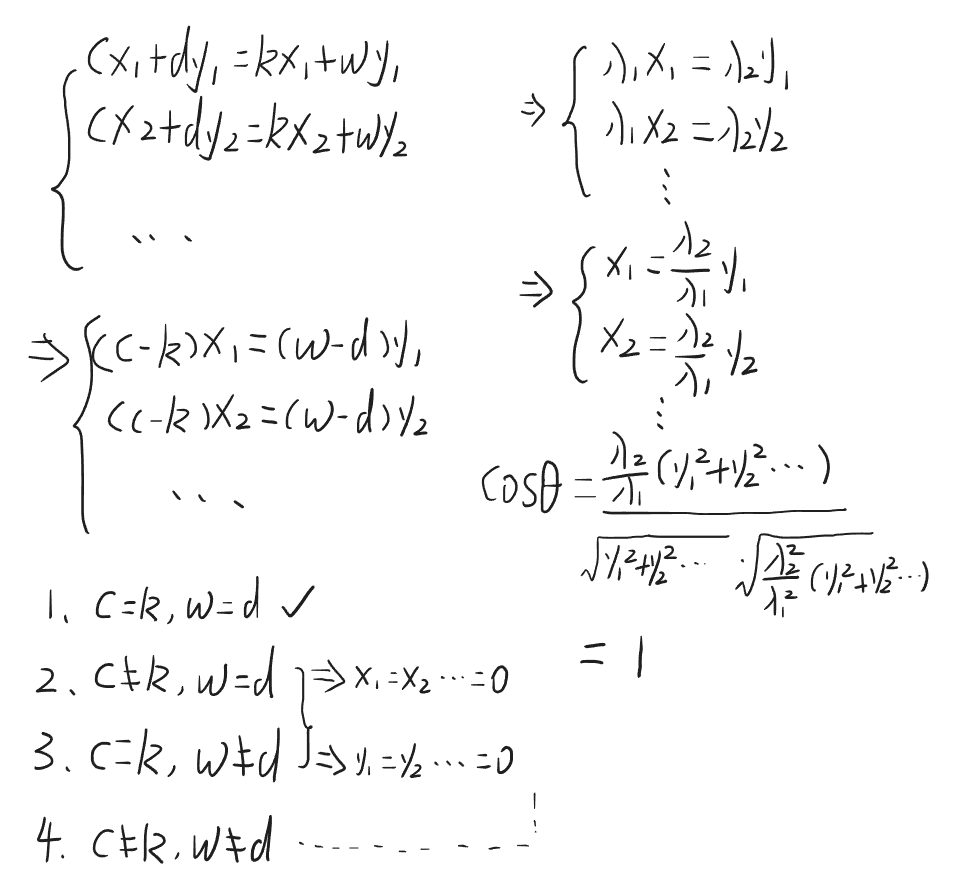
\includegraphics[width=\linewidth ,totalheight=0.95\textheight , keepaspectratio]{线性组合下向量相等的判定.png}
\caption{线性组合下向量相等的判定}
\end{figure}

上面1234四种情况,第一种情况正是我们要证明的,而第二种和第三种情况可以推出某个向量为零向量,这和条件该线性组合可以形成平面冲突。第四种情况可以证明这两个向量的夹角是零,也就是这两个向量是平行的,这也和条件冲突,于是得证。

\part{分析}












\appendix

\part{附录}
\chapter{哲学基础}
自然语言是一种很丰富多彩的语言,它的应用场景主要是针对人们的日常生活,这样的应用场景更多地是要去表达\textbf{具体的}人事物,如果有那样的表达需求,那么直接用自然语言就好了。

哲学是关于一般事物的一般规律的一般性讨论,因此自然语言中的一些词汇到了哲学领域,很多它们最终都会被认为是等价的,于是这就要求进行一些词语上表达的约定,这种表达上的约定为接下来进入更加抽象的集合论和数理逻辑等领域打下了基础;同时还存在某些概念和知识,是语言无法清晰表达的,对于这部分知识,一般是需要诉诸自然语言来尽可能地实现听众的心领神会,这一块知识是不可能诉诸某种更简单抽象的数学语言或其他形式语言的;还有哲学讨论建立了一个桥梁,如果直接就深入到更加抽象的数学术语领域,而哲学上的基础根基没有打扎实,没有对那些术语概念建立起很好的直觉,历史一次又一次地证明,这会让人们产生诸多理解困难,常常让人们犯下各种基本性的哲学错误,从而在抽象的术语迷宫中迷路。



\section{什么是物}
这里所说的物是一般意义上的物,即智能体当前的研究对象。它可以是智能体当前所处的环境,甚至还可以上升到是环境状态和智能体存在状态的综合,也可以只是其中的某一部分。

物的概念是一个高度抽象的概念,很多人会试着从视觉的角度来理解这里所说的物,但这里说的物不要求具有视觉上的那种独立分离性。

物理学家们一般会认为物的概念至少具有某种客观存在性,但这里说的物并不要求一般唯物主义观点的那种客观存在性,狭隘的唯物主义所谈论的物常常被称之为自在之物,这里说的物当然都是存在的,但不是那种狭隘的所谓自在之物的存在。

物的唯一特性是其能够或者潜在能够和智能体产生某种交互作用。可以更加精细地将那些暂时还没有和智能体交互但具有潜在交互能力的物称之为潜在之物。

\section{物的同一性}
所谓物的同一性是指智能体在和物的交互作用中,能够发现物的存在状态是相同的或不同的,并继而决定采取某种行为的能力。这种能力给予了智能体极大的生存优势,极端的筛选条件下,那些不具有某种物的同一性感知能力的智能体,将会直接被筛除掉。

要用一种更宽广的视角来看待上面的话语,上面谈到的生存优势,当然包含在真实的外部环境下的情况,但也可能只是某种虚拟的预测用环境;上面谈到的筛除,当然包含整个智能体的情况,但也可能只是智能体内部的某个部分子单元。

用数学符号表达就是 $A=B$ ,意思是A物和B物具有同一性,它们实际上指的是一个物体,只是语言表达上的一种多样性。

与之相反的:$A \neq B$ 是A和B不是同一物体的意思。


\subsection{何为智能体}
显然上面谈论的智能体不局限在人类,动物植物等生物都是所谓的智能体,继续往外扩展,某种结构稳定的物质有可能被称之为智能体\footnote{考虑到外界环境的极具破坏力,其被称为智能体应该是个大概率事件},物质当然在和外界环境发生着某种作用,如果这种结构稳定的物质在感知到能够破坏自身稳定结构的外部信息时,相应调整自身【这称之为采取了某种\emph{动作}】,从而保持自身结构的稳定性,这种物质也可以称之为智能体。


\subsection{何为交互作用}
这里说的物和智能体的交互作用是一个高度抽象的泛泛而谈的术语,或者是具体是某种物理作用;或者是智能体对于外界事物的分析观测行为;或者是智能体在环境中的某种运动等等。


\subsection{物的同一性的要求}
我有时会说智能体具有对物的同一性的感知能力,但这个感知并不是某种实在的知觉上的那种感知能力,而是一种更加抽象层面的东西,但最终的结果就是智能体确实是某种程度上,先验地无理由地感知到了物的同一性。并继而基于这种对于物的同一性感知,它首先重塑了智能体的监督组织,再继而由智能体的监督组织重塑着智能体的各个部分。

当然我没有否认智能体的感知行为的实在性,只是为了和后面要谈论的物的同一性的推理区分开来,在本小节更多地去强调智能体对于物的同一性的感知,不一定具有某种狭隘的唯物主义的实在性,而是在一个更高抽象层面上感知到了。一个简单的比方,某种具有稳定结构的物理粒子,其内部的某些行为最终将会被证实确实是有利于维持该物理粒子的稳定性的,但人们试着从物理自在规律出发来描述这种现象,可能会失望而归,对于那些狭隘的唯物主义物理学家来说,他们只有两个出路,或者接受这里讨论的物的同一性要求哲学;或者放弃解释,认为现象是这样的就是这样的。而第三条路就是试着去寻找某种额外的客观作用物理规律,最终这些尝试都将被证明是失败的。

物的同一性的要求具有极高优先级和权威性,是一种整体性思维,物的同一性要求总是正确的\footnote{这里说物的同一性要求总是正确的,是从智能体和物的交互的更高角度出发说的,不是在说智能体的监督组织一定是正确的,如果智能体的监督组织违背了物的同一性要求,那么当然该智能体也会受到惩罚。}。


\subsection{物的同一性的推理}
智能体对于物的同一性感知的发展,要求它各个部分发展出对于物的真实感知部件,从而提高感知准确度。各个部分的感知分析行为,通过某种变换、运算等等,最终得到物的同一性的结论,这个过程称之为物的同一性的推理。

物的同一性的推理是一种部分式的分析思维,是第二性的,如果物的同一性的推理和物的同一性的要求发生冲突,则物的同一性的推理将会被否定。

本章节只讨论哲学上的东西,这里说的物都是具有某种实在性的,但对于智能体在推理过程中发展出来一系列变换中间体,赋予它们某种实在性,则是一种大胆的无根据的行为。物的同一性的推理的最终目的只是为了提高物的同一性感知的准确度,去热衷于讨论这些中间过程产物的实在性也是很奇怪的。

\subsection{关于罗素的理发师悖论}
集合现在是一个推理概念了,罗素的理发师悖论促进了早期朴素集合论的自我革新。集合公理论中很重要的一条就是建立一种集合的层级关系,这是没有问题的,因为集合这个有关物的包含关系的推理演绎,如果想要逻辑自洽,就必须要做到这点,否则就会陷入死循环。

这里不是讨论数学的地方,这里提及罗素的理发师悖论,是为了说明集合公理论为什么建立那样的层级关系是合理的可行的,而且也必须是这样。其底层逻辑就是物的同一性的要求是第一性的,物的同一性推理是第二性的,如果物的同一性推理和物的同一性要求发生冲突,那么物的同一性推理将被否定。

\begin{quote}
在一个村子里,有一位理发师,他宣称自己给所有不给自己刮胡子的人刮胡子,并且只给这些人刮胡子。那么问题来了,这位理发师要不要给自己刮胡子呢?

如果理发师给自己刮胡子,按照他的原则,他只给不给自己刮胡子的人刮胡子,那么他就不应该给自己刮胡子,这就产生了矛盾。

如果理发师不给自己刮胡子,按照他的原则,他要给所有不给自己刮胡子的人刮胡子,那么他就应该给自己刮胡子,这又产生了矛盾。
\end{quote}

这个悖论犯的错误是试图从部分的推理来否定该集合整体性要求,所有不给自己刮胡子的人构成的集合,这个理发师可以在这个集合,那么他就应当服从这个整体性要求;他也可以不在这个集合;他也可以一会儿在一会儿不在,这都不是问题。

\section{无的概念}
所有的空无一物,不存在的红苹果,不存在的香蕉等等等等,所有这些表述,只是自然语言上的表述多样性,在哲学这里都是指的同一个对象,那就是\textbf{无}。数学上的零 $0$ 的概念和空集 $\emptyset$ 的概念和这里讨论的无的概念,说的都是一个对象,说的都是一回事。

无的最大特点就是智能体不可能与其产生交互作用,因此其是一个推理出来的概念【后续用语中有时会用推理抽象来描述这些概念】,因此最多仅仅从概念上将其表达出来,除此之外一切对它们的修饰描述只是词藻华丽多样,说的都是一回事,\textit{不存在}。

\section{数学是关于推理抽象的艺术}
\begin{bookref}[frametitle={\cite{Elements of Set Theory}}]
在如今的数学领域中,本质上一切事物都是一个集合。
\end{bookref}

在我看来显而易见不容反驳空集、零、无这些表达不存在的概念都是推理抽象出来的概念,智能体不可能与其发生交互作用,当我看到集合公理论的根基却是扎根于空集这个概念上时,我认识到数学上的一切概念都是推理抽象出来的概念。也就是说数学中所谈论的一些对象,从零到一等等自然数,从描述包含关系的集合到描述多个分析维度的综合的向量概念,等等等等,所有这些数学概念都是推理抽象概念。

就好像一个完整的命题,数学研究的是中间的那部分,完全脱离物的同一性,去头去尾试图将数学脱离一切独立看待终将让数学研究变得琐碎盲目和无意义。但又好像做一份完整的工作,不一定要求必须从头到尾地依次去做,你当然可以先做中间那部分,再做其余的部分,这并没有多大区别。


\subsection{为非标准分析正名}
既然所有的数学概念都是推理抽象概念,我是没看出无穷小量有什么大逆不道之处,在我看来无穷小量和圆和直线等等概念都是类似的,都属于推理抽象概念。反而在这里是要对那些为无穷小量感到不安的数学家们做点思想工作了。

有两个抽象,一个是认知抽象;一个是推理抽象。比如说人们能够认识苹果,是因为它心中有苹果的模板,这个模板心理学那边叫心理表征。继而人们会很自然地认为,人是根据看到的所有圆形的物体发展出了圆形这个认知抽象概念。从某些方面来说,确实是这样的,但关于圆形的认知抽象概念那部分不是数学家该研究的,圆形在数学家那边就是一个推理抽象概念。首先人的认知抽象是一个很复杂的领域,如上所述,其中有一些就是物的同一性要求的,先验而形成的概念,其次可能人的某些认知抽象将来会被界定为某种推理步骤,但那是将来的事情了,在这之前,要求数学家去研究那些认知抽象概念实在强人所难了。

因此有两个直线概念,一个是基于认知的,一个是基于推理的。数学家应该专注于研究基于推理的那部分。所以反而当大众对无穷小量忧心忡忡的时候,这个时候应该是数学家,这群早就习惯了各种推理抽象概念的人,站在最前面说道,引入无穷小量是合理的。


\subsection{数学上纯粹一的概念}
起初人见到苹果,早期不自觉的头脑活动使得人心中有了苹果形象和概念,但因为早期人类生存环境恶劣,并没有太多的空闲时间来发展出一二这样的纯数字概念。不过人们也已经认识到了事物的数量性质,比如基于物的同一性有如下表述:

\begin{itemize}
\item 一只手一样多的(5)
\item 人身上一样多的(20)
\end{itemize}

人类从上面的这样依靠具象事物之上的数量性质发展出 \textbf{纯粹的数学概念一} 是一个很漫长的过程。甚至某些原始部落直到近代也没有发展出纯粹数学上的一的概念,而笼统地用类似一只手那样多来表达。我以为这种纯粹数学概念一的表达出现表面上看是一种言语的精细化,抽象化,但其背后的驱动力应该来源于早期各原始部落各自独立发展出来的不同语言表达体系的碰撞。这种过程有点类似于货币的产生,有的部落将三表达为三个土豆多的,有的部落将三表达为三个苹果多的,慢慢的人们新造一个词语三来实实在在地表达事物的这个三的性质——即纯粹地数学概念三。【这里说的意思不要自大地认为很多原始部落还没有发展出数字概念,在说话的时候还需要带上某个具体的事物,认为他们好落后,实际上他们在说和人手一样多和我们现代人在说数字5的时候头脑里面想要表达的东西并无二致,只是因为他们部落可能缺乏和其他部落的沟通交流需求,所以看起来表达上略显繁琐。(这个过程叫做群体抽象过程,类似货币的最终概念确立也需要这个过程。)】

早期人们已经形成了一些纯粹数学概念上的一,五之类的词,但它们还不是如同现代数字体系那样连续的,可能还缺少某几个词。从人类发展历史来看,文字的出现是一个缓慢的过程,创造出一个文字说得出来,写的出来等等手段表达出这个概念是一回事,但头脑里是否已经有了这个概念又是另外一回事,在看待古人类发展历史这个问题,有的时候过分的自大只会妨碍了你认清事情的真相。

本小节一是承认人对于数字上一的概念最先是基于\emph{认知抽象},再继而强调原始部落,甚至那些还没有发展出纯粹数字一词汇的那些部落,他们头脑里其实也已经有了自然数的\emph{推理抽象}概念,这些和现代的数学家基于集合公理论描述的那种更加抽象的概念并无二致。最后本小节提出了\emph{群体抽象}概念,纯粹的数字词汇出现就是源自各个原始部落的沟通交流需求,从而带来的语言表达上的简化。



\section{如无必要:勿增实体}
两个相似的物体当然是可以区分开来的,但有所谓的两个同一的物体这个概念吗?

一个经典的物理问题:这个世界到底是有一个电子还是多个电子。

如果两个电子所有的性质都是一样的,当然也包括空间性质,任何观测手段都无法将其区分,那么讨论多个电子这个问题还有意义吗?或者我们只能接受这样一个事实,只存在一个电子。

这里的重点不是物理学上的讨论,而是说物的同一性这样一个事实,物体A和物体B,智能体无法区分它们的性质差异,那么应当认为物体A和物体B本质上就是同一物体,区别只是名字上的差异。

\section{如无必要:勿增关系}
\subsection{正交性}
所谓\emph{正交性},是指智能体的某个动作不影响某物的某个属性值,则称智能体的该动作与该属性存在正交性。


\subsection{动作先验正交}
在没有特别理由的情况,任何动作都应预先假设与目标属性存在正交性,并无依赖关系。即智能体认为任何动作对某物的目标属性是先验正交的。

比如小孩子懂得积木被藏在沙发底下,积木还是存在的,并没有消失。

比如铅笔被插入水中,看上去是弯的,应预先假设插水这个动作并没有改变铅笔的存在状态,然后试着修改自己对世界的观察认知。

\subsection{非正交性动作}
非正交性动作,也就是关系,即该动作能够影响某物的存在属性,之所以一般会预先假设动作和该属性具有正交性而不是确定某种关系,是因为关系的确立成本极其高昂。

一旦关系确立,智能体后续的所有类似的动作都要接受这个关系的约束,或者对该关系进行批判。

\subsection{完全正交动作}
如果某个动作不影响某物的任何属性,那么称该动作对某物是完全正交动作。在物的同一性要求的可接受范围内,可以近似认为是完全正交动作的也可以称之为完全正交动作。

以智能体的识别动作为例,识别动作对某物的某个属性值进行了识别,获取了关于该物的一些信息,应预先假设为完全正交动作。

\subsection{完全正交动作顺序无关}
有识别动作IAM和IBM分别识别某物的A属性和B属性,这两个识别动作都是完全正交动作,那么这两个识别动作发生的先后顺序不影响属性值结果输出{可能智能体具体内部细节本身就具有一定的计算并发性,但那只是具体技术细节,不影响这里的讨论。}。

按照完全正交动作的定义,这是显而易见的。


\section{等价变换}
智能体在进行物的同一性推理过程中,可以进行任意的变换、运算等等操作,如果某个操作不会改变物的同一性结论,那么这个变换称之为等价变换。

以 $A=B$ 来举例,一系列的等价变换将会构成如下序列:

\begin{align*}
A \Rightarrow a_1 \Rightarrow a_2 \Rightarrow a_3 \Rightarrow a_4 ... \Rightarrow a_n \Rightarrow B \\
B \Rightarrow a_1 \Rightarrow a_2 \Rightarrow a_3 \Rightarrow a_4 ... \Rightarrow a_n \Rightarrow A
\end{align*}

从而有:

\[
A \Leftrightarrow a_1 \Leftrightarrow a_2 \Leftrightarrow a_3 \Leftrightarrow a_4 ... \Leftrightarrow a_n \Leftrightarrow B 
\]

这样一系列的等价变换过程当然有助于智能体更好地取判断物的同一性。

这样一系列的等价变换过程可能是有限数目的,如此则称之为该等价变换族是有穷的;也可能是无穷数目的。但智能体不在乎该等价变换族是否是可以穷尽的,实际上智能体也不需要列举其中的全部,甚至智能体可以不需要主动去进行其中的某些运算【部分独立运算上报】,它需要做的就是容忍这种差异性。


\subsection{非等价变换}
不是等价变换的就是非等价变换,但不要死板地认为某类变换一定就是非等价变换。是否符合物的同一性要求是关键,确切来说,是否符合当前物的同一性判断需求,需求,是一个很灵活的词语。但非常遗憾,形而上学家们,智能体知识体系的最高标准就是这样一个灵活的需求。

有一种反驳观点,机械主义也好,形而上学家也好,会反驳到,智能体的最终物的同一性判断需求是要逼近宇宙的真相,而宇宙的真相并不是一个灵活的标准,关于这个反驳观点请继续看下面的讨论。

\subsection{学习的理想和谐态}
现在假定,智能体满足了对于物的同一性的所有需求,从而让自己在和外部世界的交互中达到了某种和谐的状态,称这样的状态是智能体达到了学习的理想和谐态。这种状态不一定是静态的,从时间的某个局部角度出发,会看到一些周期性的均衡变化,但拉长时间来看,可以近似看作无变化的了。

对于这样的观点,我是无法反驳的,我只能说考虑到世界的复杂性,小小的人类智能体是不可能穷尽彻底模拟宇宙一切可能性的,生也有涯,知无涯也。但我为什么要在这里花费一段文字来描述这样一种不可能达到的状态呢?因为这里描述的学习的理想和谐态,标记了一个方向,是有用的。

\chapter{数学基础}
\section{逻辑}
逻辑讨论了智能体的内部运作的一般性规律。所谓的数理逻辑是个奇怪的名词,仿佛逻辑只和数学或者物理有关。

逻辑上的一些基本常识,简单了解下即可,在逻辑语言的学习上,要适度,请看下面的批判。


\subsection{对形式化语言一些错误观点的批判}
\subsubsection{认为形式化语言表达能力更强}
恰恰相反,形式化语言都存在着一些约束和限定条件,表达能力最强的永远是没有限制的自然语言。


\subsubsection{认为形式化语言表达更加的精确}
认为使用形式化的语言,会更加的精确。尤其是在数学上,人们更加走向另外一个极端,会认为数学符号表达的公式会更加的精确,推荐使用 $\forall$ 这样的符号而不是 \textit{对于所有} 这样的自然语言表达。

语言,专业领域的语言,要做的只有一个工作,那就是规范化。避免出现一个人说五个苹果一样多,一个人说一巴掌一样多,大家都规范使用相同的术语方便快速沟通交流,但其实大脑在说这些不同的词语时,内部活动都是大同小异的,并没有那个会比那个更精确的说法。

\subsubsection{企图通过形式化语言的研究穷极一切真理}
假设乔姆斯基的底层语法理论是正确的,其原因只可能是因为我们都处在同一个世界之中。

假设有一个东西,存在无数种可能的变体,为什么要分析那无穷多的变体,然后隔靴搔痒地推测那个东西的存在状态,而不是直接去研究那个东西?形式化语言学家说道:是的啊,我们正要去研究那个东西,于是他们虚构出那个所谓的底层语言,并臆想到这个底层语言可能是基于基因。但是为什么不再多踏一步,是因为我们都处于同一个世界中,所以才造就了基因上运作的某种相似性,并继而造成了语言底层的某种相似性。所以为什么不直接去研究那个实在的外在世界,而要去研究某个虚构出来的底层语言呢。

本小节也是对那种研究倾向进行了批判,那就是企图通过形式化语言的研究,以一种哲学家的天真气派,想要通过大脑自身的内省活动,来穷极这世间一切的真理。这种极端的唯心主义倾向是极度有害的,当然,适度的哲学内省有时是有益的,但要适度。

\subsection{命题}
命题动作是智能体内部的描述性动作。命题动作对智能体内部存在状态是完全正交的。命题动作在人类这个智能体上会具现为命题语句,对于其他智能体则可能没有这种命题语句输出,但可以虚构出某种语言组件加之于目标研究对象上,从而产生某种虚构出来的命题语句输出行为。简便起见,命题语句简称\emph{命题},也就是上面讨论的命题动作。

一般来说智能体对自身内部存在状态相较于外部世界会更加确定明晰,对于一些无法判定的情况,这些情况不在数学的研究范围内,所以在数学上人们谈论的命题会额外加上一个条件,即智能体能够对该命题语句进行判定,判定结果只可能是真或假。这里谈及的真假,只是智能体内部认为的真或假,无关乎实际的真假。

\emph{命题成立}:所以命题成立,是指该命题可以判定真假。如果一个命题既是真又是假,那么称这个命题存在矛盾,命题不成立。


\subsection{基本命题}

\begin{description}
\item[简单命题] 不能再继续分解为某个子命题的命题称为简单命题。
\item[否定命题] 某个命题的否定称为原命题的否定命题。 $\neg A$
\item[存在命题] 类似于 \textit{D中存在具有性质E的一个对象x} 这样的命题称为存在命题。
\item[概括命题] 类似于 \textit{D中所有的对象x都具有性质E} 这样的命题称为概括命题。
\end{description}

\subsection{复合命题}
通过不同的逻辑将一些基本命题连接起来就能组成一个新的复合命题。


\subsubsection{and逻辑}
命题A和B必须都为真,复合命题才为真,否则为假。该复合命题常被称为与命题,或者合取命题。

\begin{framed}
A 且 B
\end{framed}

\begin{framed}
A and B
\end{framed}

\begin{framed}
$A \wedge B$
\end{framed}

\subsubsection{or逻辑}
命题A和B只要有一个为真则复合命题为真,否则为假。该复合命题常被称为或命题,或者析取命题。

\begin{framed}
A 或 B
\end{framed}

\begin{framed}
A or B
\end{framed}

\begin{framed}
$A \vee B$
\end{framed}

\subsubsection{异或逻辑}
命题A和B只能有一个为真复合命题才为真,否则为假。该复合命题常被称为异或命题。

\begin{framed}
要么 A 要么 B
\end{framed}

\subsubsection{if逻辑}
如果A为真B为真那么复合命题为真,如果A为真B为假那么复合命题为假,其余情况复合命题皆为真。该复合命题常被称为条件命题,或者蕴涵命题。

\begin{framed}
如果 A 则 B
\end{framed}

\begin{framed}
if A then B
\end{framed}

\begin{framed}
$A \rightarrow B$
\end{framed}

中文的蕴涵一词很让人困惑。一般会用 $A \to B$ 这样的单箭头来表示条件命题,说是为了和 $A \Rightarrow B$ 这样的推出符号区别开来,但没看出这有什么改进,仍然会让人往某种变化上联想。条件命题更多的是一种存在状态的描述,用自然语言if ... then ... 也许更能让人去把握这其中的含义。也正因为条件命题是一种静态的存在状态,所以不需要A为真来驱动推导过程,如果A为假,条件命题中的B是真是假都无所谓,反正不会触发,至于条件命题整体则不会报错总为真。



\begin{table}[H]
\begin{tabular}{@{}llllll@{}}
\toprule
{A} & {B}  & {$A \to B$} \\ \midrule

{T}          & {T}       & {T}   \\
{T}          & {F}       & {F}   \\
{F}          & {T}        & {T}   \\
{F}          & {F}       & {T}   \\ \bottomrule
\end{tabular}
\end{table}



\subsubsection{iff逻辑}
命题A和B同真同假,则复合命题为真,否则为假。该复合命题常被称为双条件命题。

\begin{framed}
A 当且仅当 B
\end{framed}

当且仅当的英文if and only if,常缩写为iff。
\begin{framed}
A iff B
\end{framed}

\begin{table}[H]
\begin{tabular}{@{}llllll@{}}
\toprule
{A} & {B}  & {$A \leftrightarrow B$} \\ \midrule
{T}          & {T}       & {T}   \\
{T}          & {F}       & {F}   \\
{F}          & {T}        & {F}   \\
{F}          & {F}       & {T}   \\ \bottomrule
\end{tabular}
\end{table}

\subsection{等价命题}
如果两个命题总是同真同假,则称这两个命题为等价命题。

\begin{equation*}
A \leftrightarrow B
\end{equation*}

如上写上一个双条件命题,并声明其为真,则其中的A命题B命题是等价命题。


\subsection{逻辑定律}
等价命题构成的双条件命题总为真。这些命题之间的变换为等价变换。

下面这些逻辑上总结出来的等价变换规律被称为逻辑定律。

\subsubsection{析取和合取的分配律}
\begin{equation}
A \text{且} (B \text{或} C) \leftrightarrow (A \text{且} B) \text{或} (A \text{且} C)
\end{equation}

\begin{equation}
A \text{或} (B \text{且} C) \leftrightarrow (A \text{或} B) \text{且} (A \text{或} C)
\end{equation}

\subsubsection{蕴涵的换位}
A成立则B成立等价于B不成立则A不成立:

\begin{equation}
(A \rightarrow B) \leftrightarrow (\text{非}B \rightarrow \text{非}A)
\end{equation}

\begin{table}[H]
\begin{tabular}{@{}llllll@{}}
\toprule
{A} & {B} & {¬A} & {¬B} & {¬B→¬A} & {A→B} \\ \midrule

{T}          & {T} & {F}  & {F}  & {T}     & {T}   \\
{T}          & {F} & {F}  & {T}  & {F}     & {F}   \\
{F}          & {T} & {T}  & {F}  & {T}     & {T}   \\
{F}          & {F} & {T}  & {T}  & {T}     & {T}   \\ \bottomrule
\end{tabular}
\end{table}

\subsubsection{析取的否定}

\subsubsection{合取的否定}

\subsubsection{存在命题的否定}
\begin{equation}
\text{非}(\exists_x | E) \leftrightarrow (\forall_x | \text{非}E)
\end{equation}

\subsubsection{概括命题的否定}
\begin{equation}
\text{非}(\forall_x | E) \leftrightarrow (\exists_x | \text{非}E)
\end{equation}

\subsubsection{蕴涵的否定}

\subsubsection{逻辑学基本定理}
如果一个命题B由假设A推出并且如果假设A被满足,那么命题B成立。

\begin{equation}
\left\{(A \rightarrow B) \text{且} A\right\} \rightarrow B
\end{equation}

\subsection{命题族}
命题族是这样一系列的命题组成的集合,它们都和目标研究物有着直接或者间接的联系\footnote{在逻辑教学书籍上喜欢将苏格拉底会死的和苹果是红的等一些毫不相关的命题组合起来的做法是很奇怪的。},它们或真或假,但都彼此之间是逻辑自洽的,即在命题族内所有的命题都是成立的。

命题族很好地描述了智能体关于目标研究物的内部认知状态。




\section{集合}
\subsection{集合的同一性判定}
集合的同一性判定,对应数学集合论的外延公理:对于A,B两个集合,对任意物体t,都有 $t \in A$ 当且仅当 $t \in B$ ,则有 $A=B$ 。

外延公理定义了两个集合判断同一性的方法,即两个同一的集合,它们拥有完全相同的成员。

对于该集合来说,A和B只是不同的名字,仅此而已。因此外延公理的反向推理也是必然成立的,A和B本质上就是一个物体,所以必然对于任意的物体t,都有 $t \in A$ 当且仅当 $t \in B$ 。


\subsection{集合内元素无顺序}
$\{x, y\} =\{y, x\}$ 这两个集合是同一的,这里并不是要否认物的空间顺序属性,比如前面的例子,x和y区别就是x是左手,y是右手,x和y成员的区别,顺序属性是其自身携带的,并不随集合的写法而转变,集合不自带顺序属性。

\subsection{集合内元素无计数}
请看下面的写法:$\{x, x\}$ ,按照物的同一性定义,x是相同的物,这种写两个x的写法是无意义的,应该归约为 $\{x\}$ 。




\chapter{术语}
\section{恒等于}
$A \equiv B$ 表示A恒等于B。恒等于仍然是属于 $A=B$的概念范畴,即A和B都是指一个东西。而恒等于是更加精细的等于的说法,A恒等于B的意思是这里仅仅只是用到了一些名称缩写或其他名字上的变化规则,在这里没有任何新的数学知识引入进来。

\section{定义等于}
$A := B$ 表示A定义等于B。定义等于仍然属于 $A=B$的概念范畴,只是更加精细地表明了在这里是先验地定义或者说假定这个语句为真。比如说 $x := x*x$ ,该语句的意思是假定x的值被定义等于其自身的平方。在后续的讨论中$x$当然等于$x*x$,只是更加精细地指出这个等于语句是先被假定为真的。





\section{自然数集}
本书认为0不属于自然数集,当本书讨论自然数集 $ \mathbb{N} $的时候,等于正整数集 $\mathbb{N}^{*}$,即:

\[
\mathbb{N} \equiv \mathbb{N}^{*}
\]

之所以本书认为0不是自然数,一是哲学上讨论的一脉相承;另外就是本书将自然数放在对数字介绍的第一部分,后面才慢慢将数系扩展开来,因此第一部分尽可能地简单为好;再就是从数学的发展历史来看,零也确实是后面才出现的纯粹数。

\chapter{约定}
向量一般默认为列向量。可以写为 $(x_1, x_2...)$ 或者 :

\[
\begin{bmatrix}x_{1}  \\ x_2 \\ \vdots \end{bmatrix}
\]

行向量则写为 $[x_1, x_2...]$


\chapter{其他}

\subsection{问题集1.1第6题}
\cite{线性代数引论}问题集1.1第6题,作者内心一个潜藏的推理思路是:如果向量的线性组合,可以从中发现某些普遍规律,也就是找到某种关系,使得这个关系不依赖参数c、d...等,那么这个普遍规律对于该线性组合下的所有点都是成立了。【我们太习惯某个事物的局部或者某些特殊情况会更简单一些,常常会忘了在某些时候(这种情况确实很罕见,但也是存在的),该事物从全局从一般情况思考会更简单一些,发现一些普适性的规律,然后自然那些局部的点特殊的情况也一应得到证明了。】

\subsection{问题集1.1第15题}
\cite{线性代数引论}问题集1.1第15题的 $\frac{3}{4}\boldsymbol{v} + \frac{1}{4}\boldsymbol{w}$ 为什么一定在对角线上,证明如下:

\begin{figure}[H]
\centering
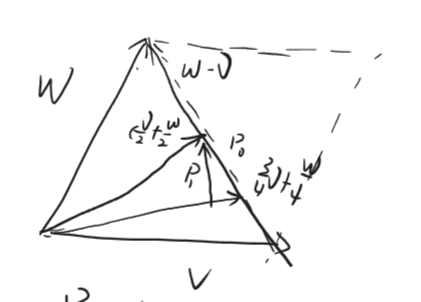
\includegraphics[width=\linewidth ,totalheight=0.95\textheight , keepaspectratio]{线性代数引论问题集1_1_15.png}
\caption{线性代数引论问题集1.1.15}
\end{figure}

已知该对角线为 $\boldsymbol{w} - \boldsymbol{v}$,标记该向量为 $P_0$,现在假定$\frac{3}{4}\boldsymbol{v} + \frac{1}{4}\boldsymbol{w}$ 射出去之后并没有落在对角线上,从而根据$\frac{1}{2}\boldsymbol{v} + \frac{1}{2}\boldsymbol{w}$ 和$\frac{3}{4}\boldsymbol{v} + \frac{1}{4}\boldsymbol{w}$ 的终点确立向量 $P_1$。【已经证明了$\frac{1}{2}\boldsymbol{v} + \frac{1}{2}\boldsymbol{w}$的终点是落在那条对角线的中点的,这很简单,用简单的三角几何分析即可。】

\begin{align*}
P_1 &= \frac{v}{2} + \frac{w}{2} - (\frac{3v}{4} + \frac{w}{4}) \\
    &= -\frac{1}{4}v + \frac{w}{4} \\
    &= \frac{1}{4}(w-v) \\    
 => P_1 // P_0
\end{align*}

因为 $\frac{1}{2}\boldsymbol{v} + \frac{1}{2}\boldsymbol{w}$ 在那条对角线的上,所以 $\frac{3}{4}\boldsymbol{v} + \frac{1}{4}\boldsymbol{w}$ 一定在这条对角线上。上面的证明过程还证明了 $P_1$ 的长度是1/4对角线长度,其终点位置刚好是对角线下面1/4的位置。

上面的证明还可以继续推广,问向量$\boldsymbol{v}$和向量$\boldsymbol{w}$组成的线性组合$c\boldsymbol{v} + d\boldsymbol{w}$ ,$c$和$d$满足何种约束条件就能让其都落在中间那条对角线也就是 $\boldsymbol{w} - \boldsymbol{v}$ 上。

证明如下,其中用到了上面提及的线性组合下向量相等的判定:

\begin{figure}[H]
\centering
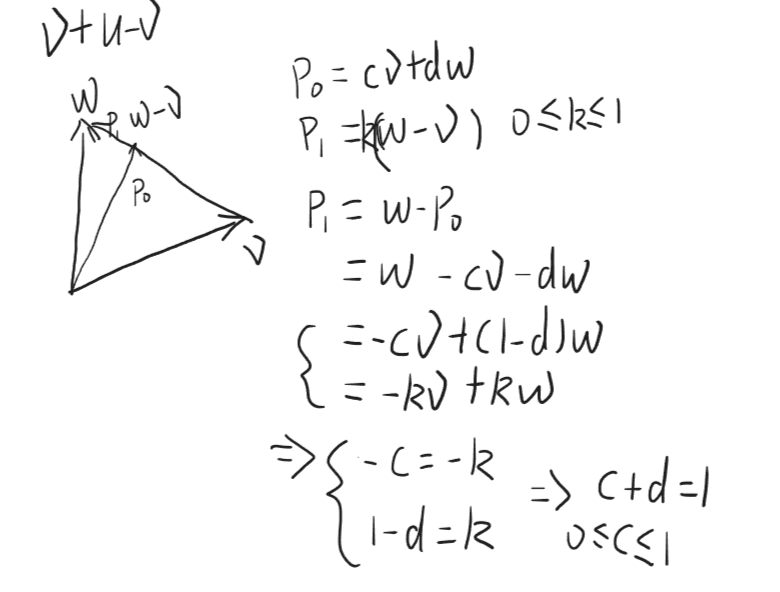
\includegraphics[width=\linewidth ,totalheight=0.95\textheight , keepaspectratio]{线性代数引论问题集1_1_15_2.png}
\end{figure}

最终得证:向量 $P_0 = c\boldsymbol{v}+d\boldsymbol{w}$ ,该向量如果满足 $c+d=1$的条件,则射出去的向量落点会落在中间那条对角线上。


\cite{线性代数引论}问题集1.1第20题将上面讨论的情况扩展到了三个向量的线性组合,问这三个向量的线性组合中,某个向量的系数满足何种条件,该向量的落点在这三个向量终点构成的三角形平面上,有了前面的基础,就很容易得证了。


\begin{figure}[H]
\centering
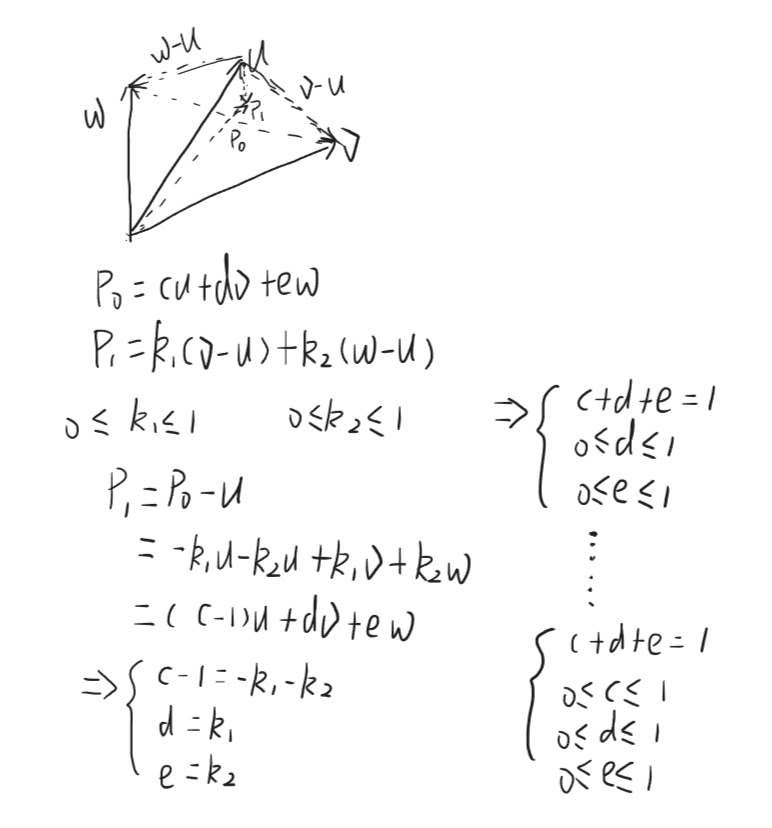
\includegraphics[width=\linewidth ,totalheight=0.95\textheight , keepaspectratio]{线性代数引论问题集1_1_20.png}
\end{figure}



\backmatter
\part*{参考资料}
\begin{thebibliography}{99}
\bibitem[什么是数学]{什么是数学} 《什么是数学:对思想和方法的基本研究(第三版)》 by [美] R·柯朗 \& H·罗宾 \&  左平[译]  at 2012.
\bibitem[高观点下的初等数学第一卷]{高观点下的初等数学第一卷} 《高观点下的初等数学(第一卷)》by [德]菲利克斯·克莱因 \& 舒湘芹[译] at 2008.
\bibitem[数学指南]{数学指南} 《数学指南:实用数学手册》 by [德]埃伯哈德·蔡德勒 at 2012. 
\bibitem[古今数学思想]{古今数学思想} 《古今数学思想》by [美]莫里斯·克莱因 at 2013.
\bibitem[烧掉数学书]{烧掉数学书} 《烧掉数学书:重新发明数学》by [美]杰森·威尔克斯 \& 唐璐[译] at 2020.
\bibitem[近似计算初步]{近似计算初步} 《近似计算初步》by 余元希 at 1961.
\bibitem[理论和实用算术]{理论和实用算术} 《初等数学教程:理论和实用算术》by [法]唐乃尔 \& 朱德祥[译] at 2011.
\bibitem[普林斯顿概率论读本]{普林斯顿概率论读本} 《普林斯顿概率论读本》by [美]史蒂文·J. 米勒 at 2020.
\bibitem[Elements of Set Theory]{Elements of Set Theory} 《Elements of Set Theory》by Herbert B. Enderton at 1977.
\bibitem[线性代数引论]{线性代数引论} 《Introduction to Linear Algebra 5e》 by Gilbert Strang at 2016 .
\end{thebibliography}
\end{document}


